%\clearpage

%\section{Background Estimation Technique}

The dominant background to the signal sample comes from \ttll\
events. Due to the presence of a second neutrino, \ttll\ events do
not have a kinematic edge at $\mt \sim \mW$. These events satisfy the
selection criteria due to real \met\ and do not depend on detector
resolution or \met\ mis-measurement effects. As a result, the
\ttll\ background is expected to be well modeled in the MC. The
prediction for this background is thus derived from MC and normalized
to the data in the \mt\ peak region. However,
there are two aspects that require dedicated corrections and are detailed
in this section:
\begin{itemize}
\item the modeling of additional jets from radiation, required to satisfy the 4-jet
selection criteria.
\item the modeling of the isolated track veto efficiency, which is
  applied to explicitly reject leptons from \W\ and $\W\To\tau$ decays
  and single prong $\tau$ decays.
\end{itemize}
The systematic uncertainty associated with the MC prediction then has two components.
One that is
derived by comparing various generators, and a second from the uncertainties on
the various correction factors used. These are described at the end of
this section.  


\subsubsection{Normalization of the Top Prediction}
\label{sec:topnorm}

In this section we discuss the factor $ {N_{peak}^{data} \over N_{peak}^{MC}} $ in Equation XX.
The same factor is applied to both the single and dilepton estimates.

The overall normalization of the \ttbar\ sample is determined by
scaling to the \mt\ peak control region, following a procedure similar 
to that described in Section.~\ref{sec:bkg_singlelep}. This control
region is dominated by \ttbar\, albeit in its single lepton decay
mode. The basic idea is that after adjusting the modeling of
additional jets from radiation in the \ttll\ sample and correcting  
the leptonic branching fractions in the \ttbar\ sample, the MC 
prediction for the \ttlj\ and \ttll\ samples is subject to the same
sources of uncertainty: the \ttbar\ cross section, the luminosity, the
selection efficiencies, etc$\dots$ The exception is the veto on events
containing an isolated track, since this last requirement has a different 
impact on the \ttlj\ and \ttll\ samples. The impact of this
requirement is addressed separately in Section.~\ref{sec:trkveto}. 

The \mt-peak scale factor is thus determined after applying the full
analysis selection with the exception of the isolated track veto. 
Specifically, the pre-veto sample is defined by the following requirements
\begin{itemize}
\item At least 1 selected electron (muon) with \pt $>$ 30 GeV and $|\eta|<2.5$ ($|\eta|<2.1$)
\item At least 4 selected jets, of which at least 1 is b-tagged
\item \met\ $>$ 100 GeV 
\end{itemize}

%As in the case of the single lepton + jets sample, 
Scaling the overall 
normalization to the \mt\ peak largely reduces the dependence on the
\ttbar\ cross section and cancels systematic uncertainties associated
with effects such as the luminosity, selection efficiencies,
etc$\dots$ However, the \mt\ peak control sample is contaminated 
by non-\ttbar\ processes, particularly \wjets\ that contributes at
the $5-10\%$ level, even after requiring a b-tagged jet. The \wjets+HF
process is a particular concern given the large theoretical
uncertainties associated with their production. 
Therefore a systematic uncertainty is derived to account for
the uncertainty in this background component. The normalization of 
the \wjets\ sample is scaled up and down by $50\%$ and the full 
background estimate recomputed. 

It should be noted that the background prediction obtained using
the same normalization scale factor based on the \mt\ peak for the 
single lepton and dilepton samples is subject to smaller uncertainties
than the prediction obtained by normalizing the \ttll\ component alone
to the overall yield in the two-lepton control sample. The reason is 
that the normalization of the two-lepton control yield depends on
effects that do not impact the \ttll\ sample with one reconstructed
lepton (i.e. the signal sample of interest) in the same way. Example
of these effects include the dilepton trigger and second lepton
reconstruction efficiencies.

In conclusion, the pre-veto sample is used to define an overall data
over MC scale factor ($SF^{\rm{all}}$) in the \mt\ peak control region, that is
applied to all background predictions and is simply defined as
\begin{itemize}
\item $N_{\rm{peak}}^{\rm{all}}$ = data yield in the peak region $60<\mt<100$ GeV
\item $M_{\rm{peak}}^{\rm{all}}$ = MC yield in the peak region $60<\mt<100$ GeV
\item $SF^{\rm{all}} = N_{\rm{peak}}^{\rm{all}} / M_{\rm{peak}}^{\rm{all}}$
\end{itemize}
For all subsequent steps, the scale factor $SF^{\rm{all}}$ is applied to all MC contributions.

\subsubsection{The Isolated Track Veto}
\label{sec:trkveto}

In this section we discuss the factors 
${(1- \epsilon_{fake})^{data} \over (1 - \epsilon_{fake})^{MC}} $
and
${(1- \epsilon_{iso\ trk})^{data} \over (1 - \epsilon_{iso\ trk})^{MC}} $
in Equation XXX.

The \ttll\ background is further suppressed after the $4$-jet
requirement by removing events with any isolated track with 
$\pt>10~\GeV$. 
%
As isolation definition we use
relative track isolation $\sum \pt/\pt(trk)$ in a cone of size $R=0.3<0.1$. 
%
This isolated track veto rejects events with an 
\E\ or a \M, as well as single-prong $\tau$-decays. 
This veto is very effective at reducing the dilepton background. In
particular, according to the \ttll\ MC, the veto removes about
three-quarters of events with an \E\ or \M\ from the \W\ decay and
almost half the leptonic and single prong $\tau$
decays. The veto has no impact on multi-prong $\tau$s, though this is
a smaller component overall. Since the \ttll\ background includes
different types of processes, it is useful to first characterize the
composition of this background. 

\subsubsection{Top Dilepton Sample Composition}

The \ttll\ background may be categorized based on the type of
second lepton, as shown in Table.~\ref{tab:ttdlcomposition}. The main
component is from electrons and muons from a \W\ decay or through an
intermediate $\tau$ decay. The second largest component arises from
single-prong hadronic $\tau$ decays, followed by multi-prong
$\tau$s. Finally an additional contribution arises from leptons
falling in the forward region, outside the Tracker acceptance
$|\eta|>2.5$ (refered to as `lost').

\begin{table}[!ht]
\begin{center}
\begin{tabular}{l|c|c}
\hline
            Sample					&                Yield   & 	Fraction [\%]\\
\hline
\hline
$t\bar{t} \rightarrow l^{+}l^{-} (\mathrm{lost})$   &       7 $\pm$ 1 	& 	6\\
$t\bar{t} \rightarrow l^{+}l^{-} (e/\mu)$   &      30 $\pm$ 3  	& 26\\
$t\bar{t} \rightarrow l^{+}l^{-} (\tau_{\mathrm{lep}})$   &      21 $\pm$ 2  	& 18\\
$t\bar{t} \rightarrow l^{+}l^{-} (\tau_{\mathrm{had}}\rightarrow \mathrm{1-prong})$   &      39 $\pm$ 3  & 34\\
$t\bar{t} \rightarrow l^{+}l^{-} (\tau_{\mathrm{had}}\rightarrow \mathrm{3-prong})$   &      19 $\pm$ 2  & 16\\
\hline
         total $t\bar{t} \rightarrow l^{+}l^{-} $  &     117 $\pm$ 5  & 100\\
\hline
\end{tabular}
\caption{Dilepton events satisfying the full selection criteria
 and \met\ $>$ 100 GeV, \mt\ $>$ 150 GeV,  separated by decay modes.
Recall that \ttll\ accounts for $\approx80$\% of the total background.{\bf Fix me: Is this before or after the isolated track veto?}
\label{tab:ttdlcomposition}}
\end{center}
\end{table}

The isolated track veto does not apply to the components where the
second lepton falls outside the acceptance or where it decays to a 
hadronic tau that is not explicitly rejected. For the cases where the
second lepton includes an electron or muon or a charged $\pi/K$, it is
possible to further distinguish cases when the relevant particle
targeted by the veto is below the \pt\ threshold. Matching the
truth-level particle to reconstructed tracks shows that in \ttll\ MC
\begin{itemize}
\item for $t\bar{t} \rightarrow l^{+}l^{-} (e/\mu)$, about a third of
  the sample falls below the \pt\ threshold of the track veto, and the remaining 
  two thirds fail the isolation
\item for $t\bar{t} \rightarrow l^{+}l^{-} (\tau_{\mathrm{lep}})$,
  about $80\%$ are soft $\pt<10~\GeV$ and about $20\%$ are
  non-isolated
\item for $t\bar{t} \rightarrow l^{+}l^{-}
  (\tau_{\mathrm{had}}\rightarrow \mathrm{1-prong})$, 
about $70\%$ are soft, as expected from a $\tau$ decay product and the
rest fail the isolation criteria.
\end{itemize}
In summary, the combination of these fractions with the relative sample
composition listed in Table.~\ref{tab:ttdlcomposition} shows that only
about a third of the \ttll\ background sample is from 2nd leptons (e, $\mu$, or $\tau\to$1-prong)
which satisfy \pt\ $>$ 10 GeV but fail the track isolation criterion
veto\footnote{Explicitly, the fraction of events that give rise to a
  sufficiently energetic lepton or single prong $\tau$ is: $70\%$ of \E-\M\ events
  which are $26\%$ of the sample, $20\%$ of leptonic tau events which
  are $18\%$ of the sample and $30\%$ of single prong $\tau$ events 
  which are $10\%$ of the sample.}. The performance of the isolation
used in the track veto requirement is the subject of the next section.

It should also be noted that according to the MC, track reconstruction 
inefficiencies affect a few percent ($\sim 1-2\%$) of the
leptonic and single prong $\tau$ events. The tracking efficiency in
this analysis is taken from MC, which is expected to provide good modeling of isolated 
tracks with $\pt>10~\GeV$. The impact of  
possible differences between data and MC is found to be negligible. 
In particular, the case of single-prong taus is the most challenging to
model due to the effect of nuclear interactions in the tracker material. 
Past studies of the tracking efficiency for pions~\cite{TRK10002}
provide a data/MC uncertainty in the tracking efficiency of $3.9\%$\footnote{
This tracking efficiency uncertainty estimate is conservative for this 
analysis since it includes tracks of \pt\ down to $250$ MeV, where
material effects are larger and so are the corresponding
uncertainties.}. Propagating this uncertainty to the total background
estimate yields a total uncertainty of $< 0.5\%$. The reason is that
the tracking efficiency uncertainty only applies to single prong
$\tau$ decays with $\pt> 10~\GeV$, which are under $30\%$ of the 
dilepton component, which in turn is $\sim 80\%$ of the total sample.  

To conclude, the \ttll\ background arises from events where the second
lepton falls outside the acceptance (both in $\eta$ and $\pt$),
because the event contains a hadronic tau that is not explicitly rejected or
because the second lepton fails the isolation requirement. 
Even though the \ttll\ sample is quite heterogenous and comprises
multiple types of second lepton events, there are two
main sources of uncertainty in this estimate: 
\begin{itemize}
\item Acceptance effects, which are estimated by using alternative MC
  samples. Here acceptance refers to the combination of $\eta$ and \pt of the leptons.
\item Detector effects, mainly arising from understanding the
  performance of the isolated track veto, which impacts only about a
  third of the total \ttll\ sample.
\end{itemize}


\subsubsection{Summary of the \ttdl\ Background Estimation Procedure}

The SM background in the signal region, defined by requirements of
large \met\ and \mt, is estimated using MC. The MC is validated using
data control samples, which are used to derive data-to-MC scale 
factors and corresponding uncertainties.

The procedure to estimate the background prediction may be summarized
as
\begin{itemize}
\item Apply the state-of-the-art corrections to the MC, reflecting the
  best knowlege of the detector performance, in order to improve the agreement
  with the data. This includes effects such as the modeling of the pileup, the jet energy scale,
  \met\ corrections, etc$\dots$ 
\item Correct the leptonic branching fractions in the \ttbar\ MC
\item Use the dilepton sample with two selected leptons to reweight
  the \njets\ distribution in \ttll\ MC, which is not necessarily
  well-modeled due to the presence of additional jets from radiation.
\item Use the pre-veto sample (i.e. applying the full analysis selection
  with the exception of the isolated track veto) to define a scale
  factor in the \mt\ peak region. This scale factor corrects for
  effects of integrated luminosity, \ttbar\ cross section, lepton
  selection and trigger efficiencies.
\item Correct the \ttll\ sample for differences between data and MC in the isolation for
  events with a second lepton. This correction is derived using $\Z+4$
  jet events and applied to the \ttll\ sample. 
\item In the signal sample, after applying the full selection
  including the isolated track veto, derive a scale factor to
  account for possible data vs. MC discrepancies in the isolated track 
  fake rate for backgrounds which have a single genuine lepton. This
  scale factor is applied to the single lepton backgrounds only.
\end{itemize}


\clearpage

\subsection{Check of MC modelling of \ttdl}


[EXPLAIN THE CROSS CHECKS DONE TO VALIDATE THE MC MODELLING OF \ttdl]

\subsubsection{Validation of the ``Physics'' Modelling of the \ttdl\ MC}

[EXPLAIN ALL THE CR4 2-lepton \ttdl\ SAMPLE ]

\begin{table}[!h]
\begin{center}
\begin{tabular}{l||c|c|c|c}
\hline
Sample              & CR4A & CR4B & CR4C & CR4D \\
\hline
\hline
Muon Data/MC-SF 	  & $0.91 \pm 0.04$ & $0.94 \pm 0.07$ & $1.06 \pm 0.13$ & $1.03 \pm 0.22$ \\
\hline
\hline
Electron Data/MC-SF 	  & $0.95 \pm 0.04$ & $1.00 \pm 0.08$ & $0.85 \pm 0.12$ & $0.83 \pm 0.19$ \\
\hline
\end{tabular}
\caption{ Data/MC scale factors for total yields, applied to compare
  the shapes of the distributions.
  The uncertainties are statistical only.
\label{tab:cr4mtsf}}
\end{center}
\end{table}


\begin{table}[!h]
\begin{center}
\begin{tabular}{l||c|c|c|c}
\hline
Sample              & CR4A & CR4B & CR4C & CR4D \\
\hline
\hline
Muon MC 		  & $199 \pm 7$ & $102 \pm 6$ & $29 \pm 3$ & $8 \pm 1$ \\
Muon Data 		  & $187$ & $108$ & $34$ & $9$ \\
\hline
Muon Data/MC SF 	  & $0.94 \pm 0.08$ & $1.06 \pm 0.12$ & $1.17 \pm 0.23$ & $1.09 \pm 0.40$ \\
\hline
\hline
Electron MC 		  & $203 \pm 8$ & $97 \pm 5$ & $26 \pm 2$ & $8 \pm 1$ \\
Electron Data 		  & $201$ & $102$ & $25$ & $5$ \\
\hline
Electron Data/MC SF 	  & $0.99 \pm 0.08$ & $1.06 \pm 0.12$ & $0.97 \pm 0.21$ & $0.60 \pm 0.29$ \\
\hline
\end{tabular}
\caption{ Yields in \mt\ tail comparing the MC prediction (after
  applying SFs) to data. The uncertainties are statistical only.
\label{tab:cr4yields}}
\end{center}
\end{table}

\begin{figure}[hbt]
  \begin{center}
	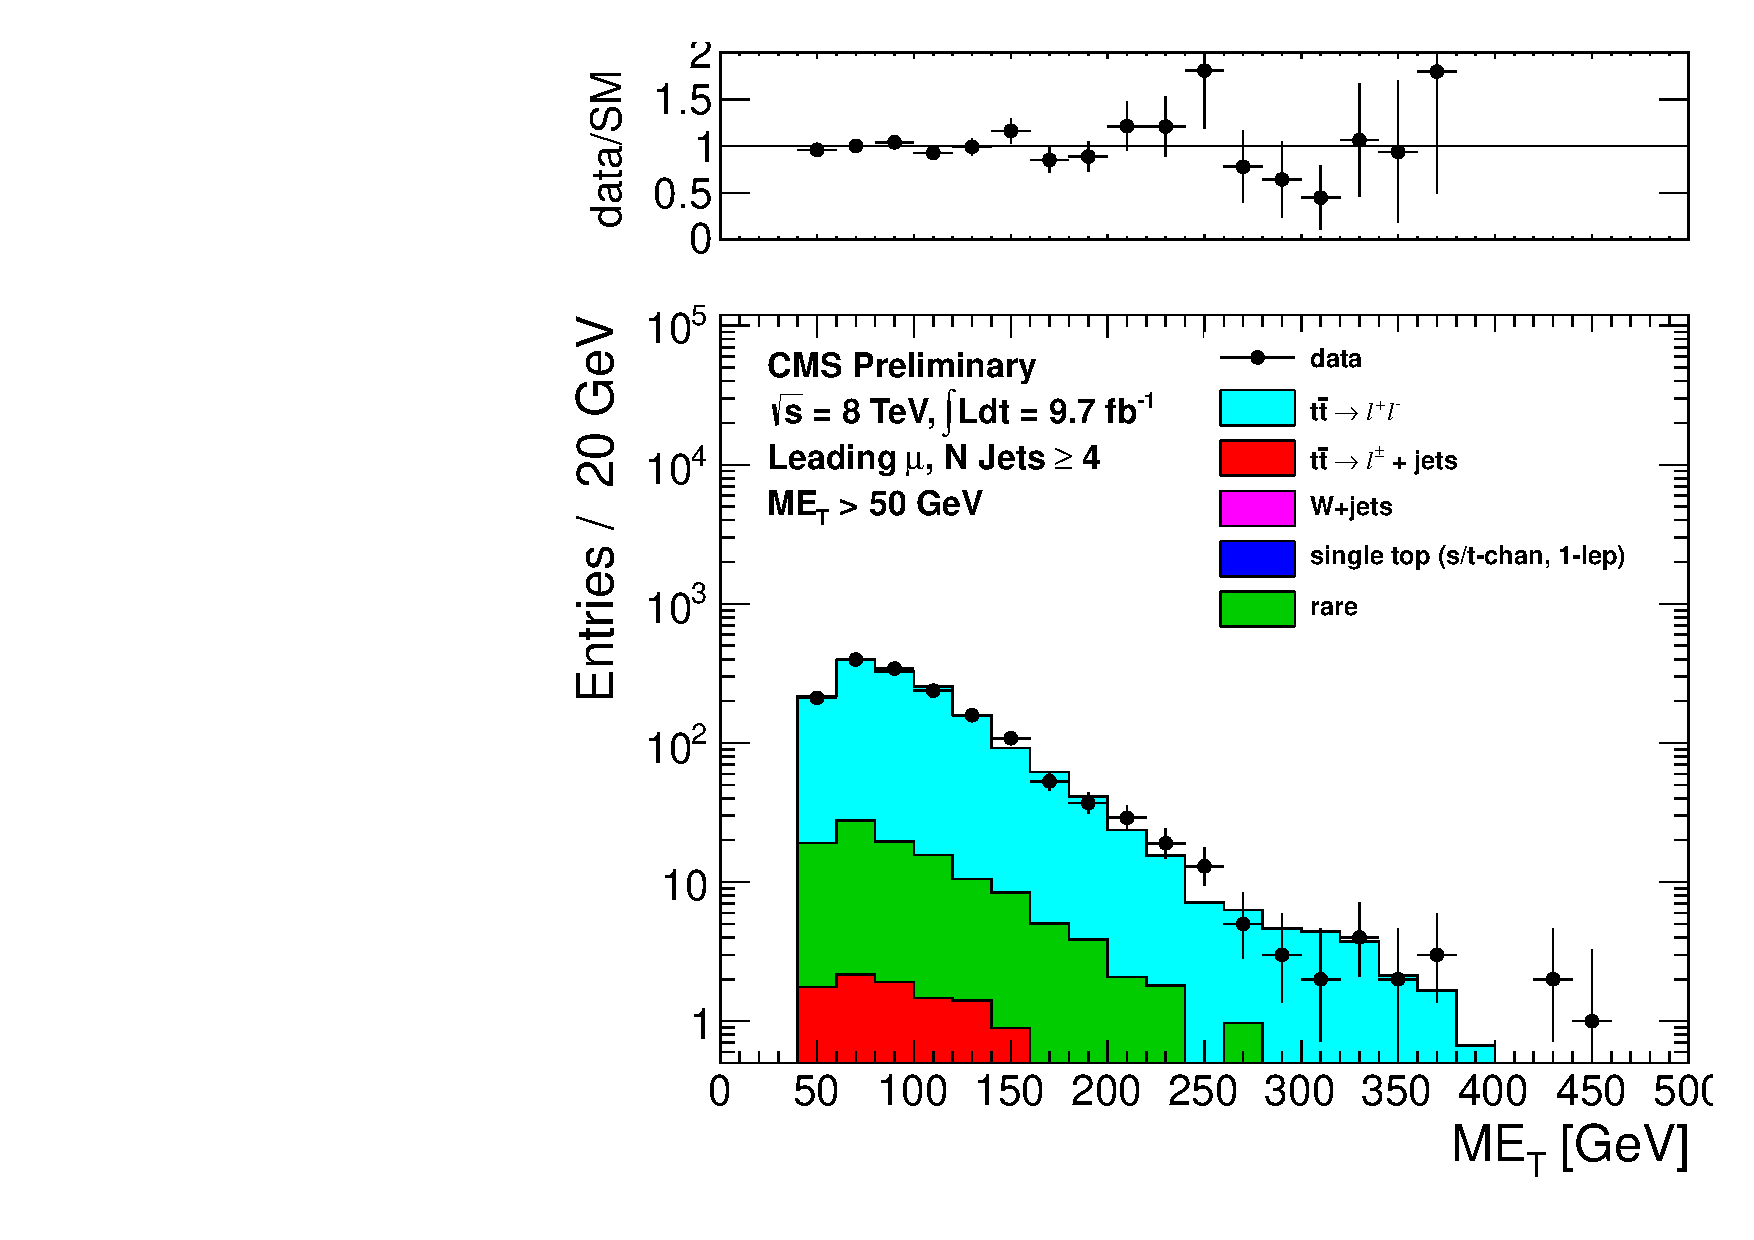
\includegraphics[width=0.5\linewidth]{plots/CR4plots/met_met50_leadmuo_nj4.pdf}%
	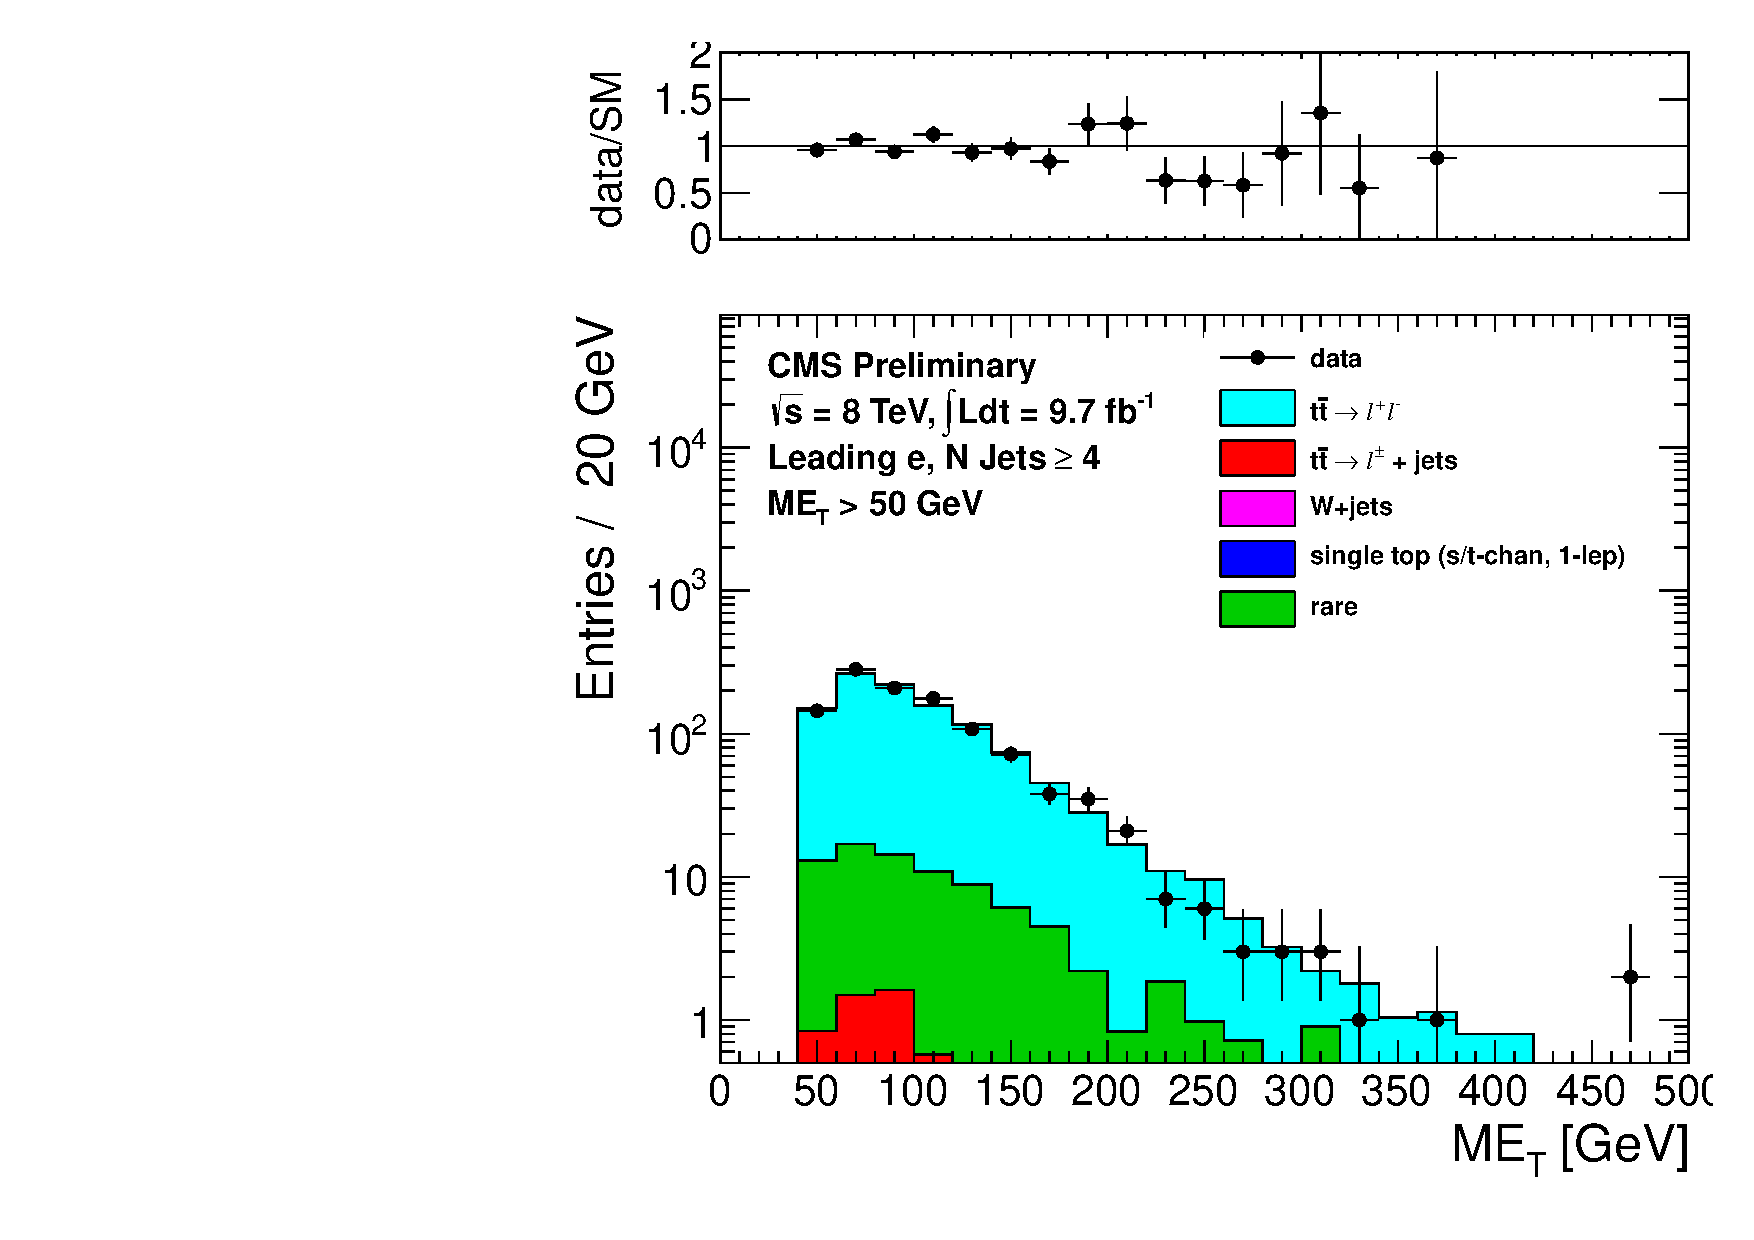
\includegraphics[width=0.5\linewidth]{plots/CR4plots/met_met50_leadele_nj4.pdf}
	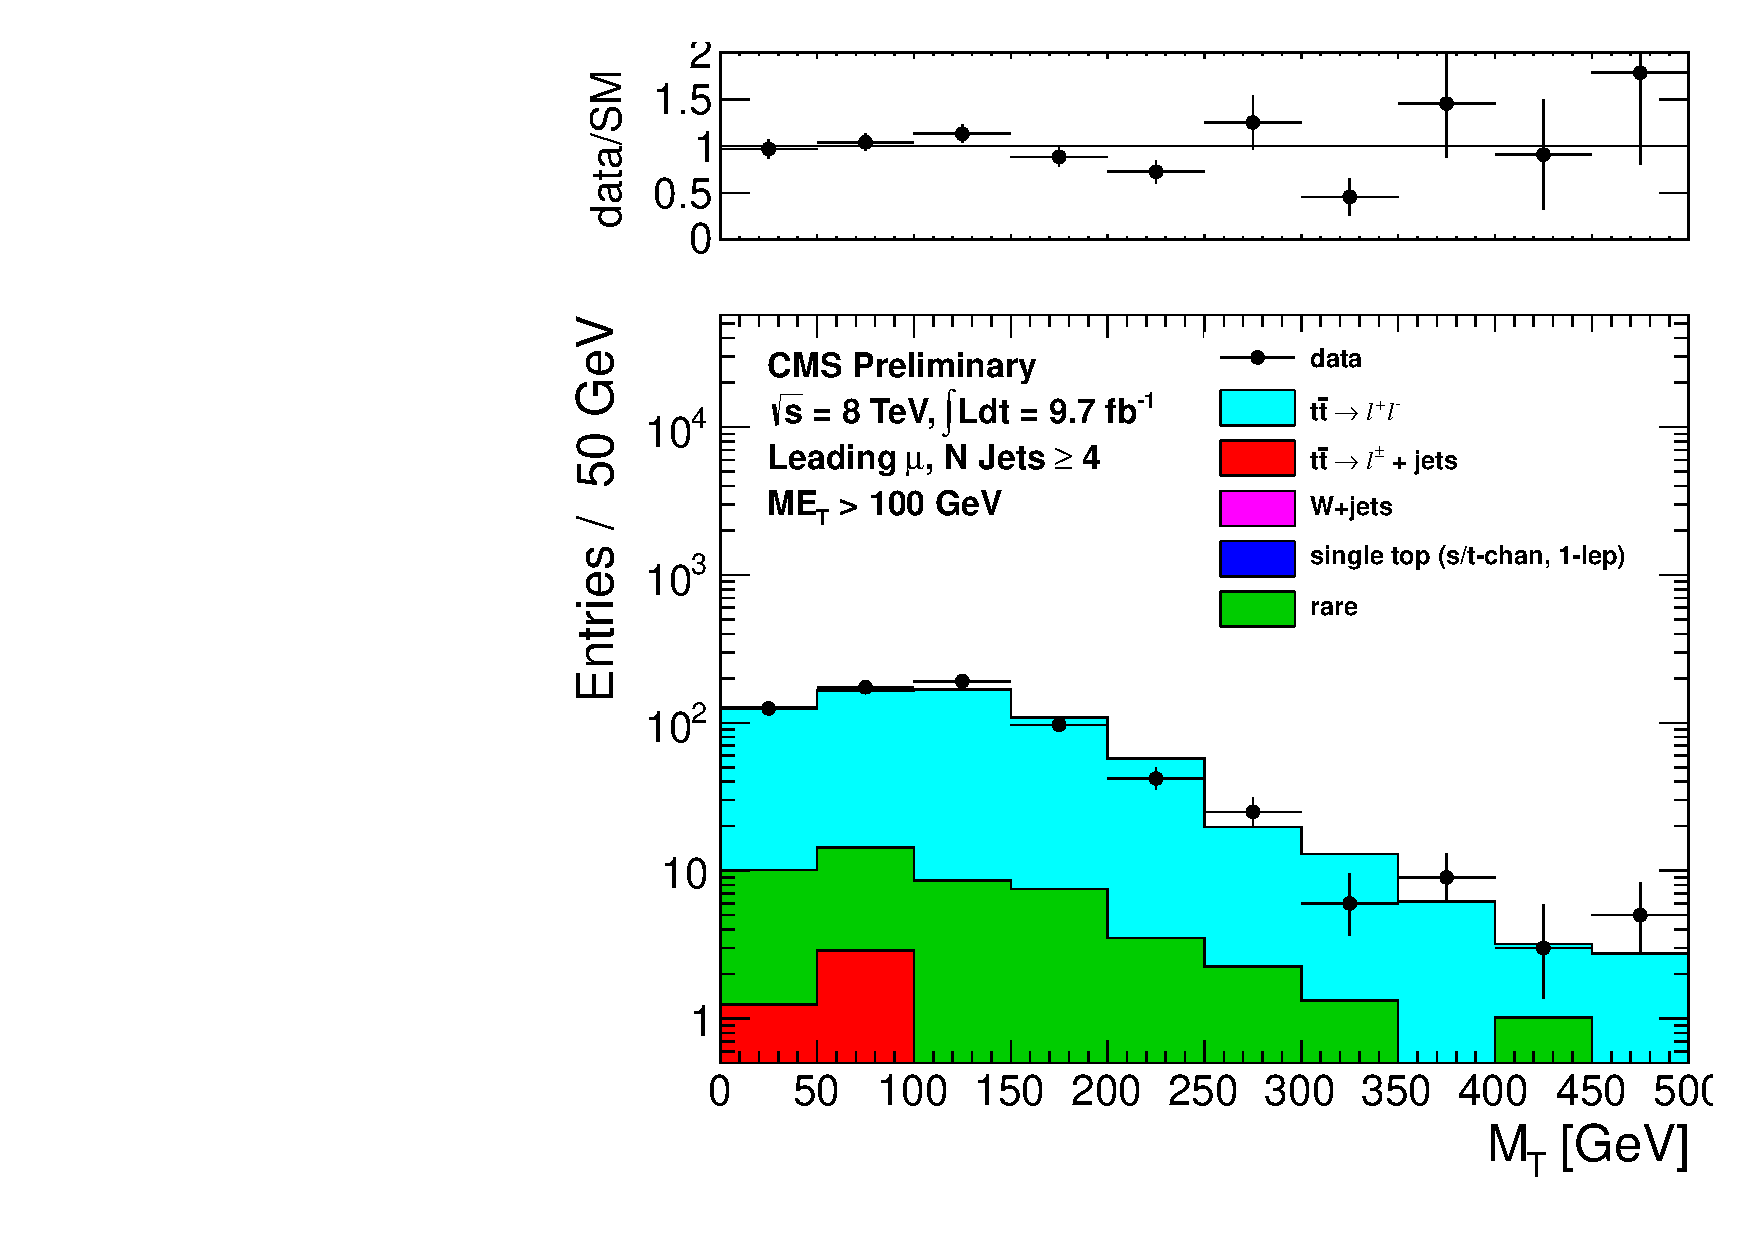
\includegraphics[width=0.5\linewidth]{plots/CR4plots/mt_met100_leadmuo_nj4.pdf}%
	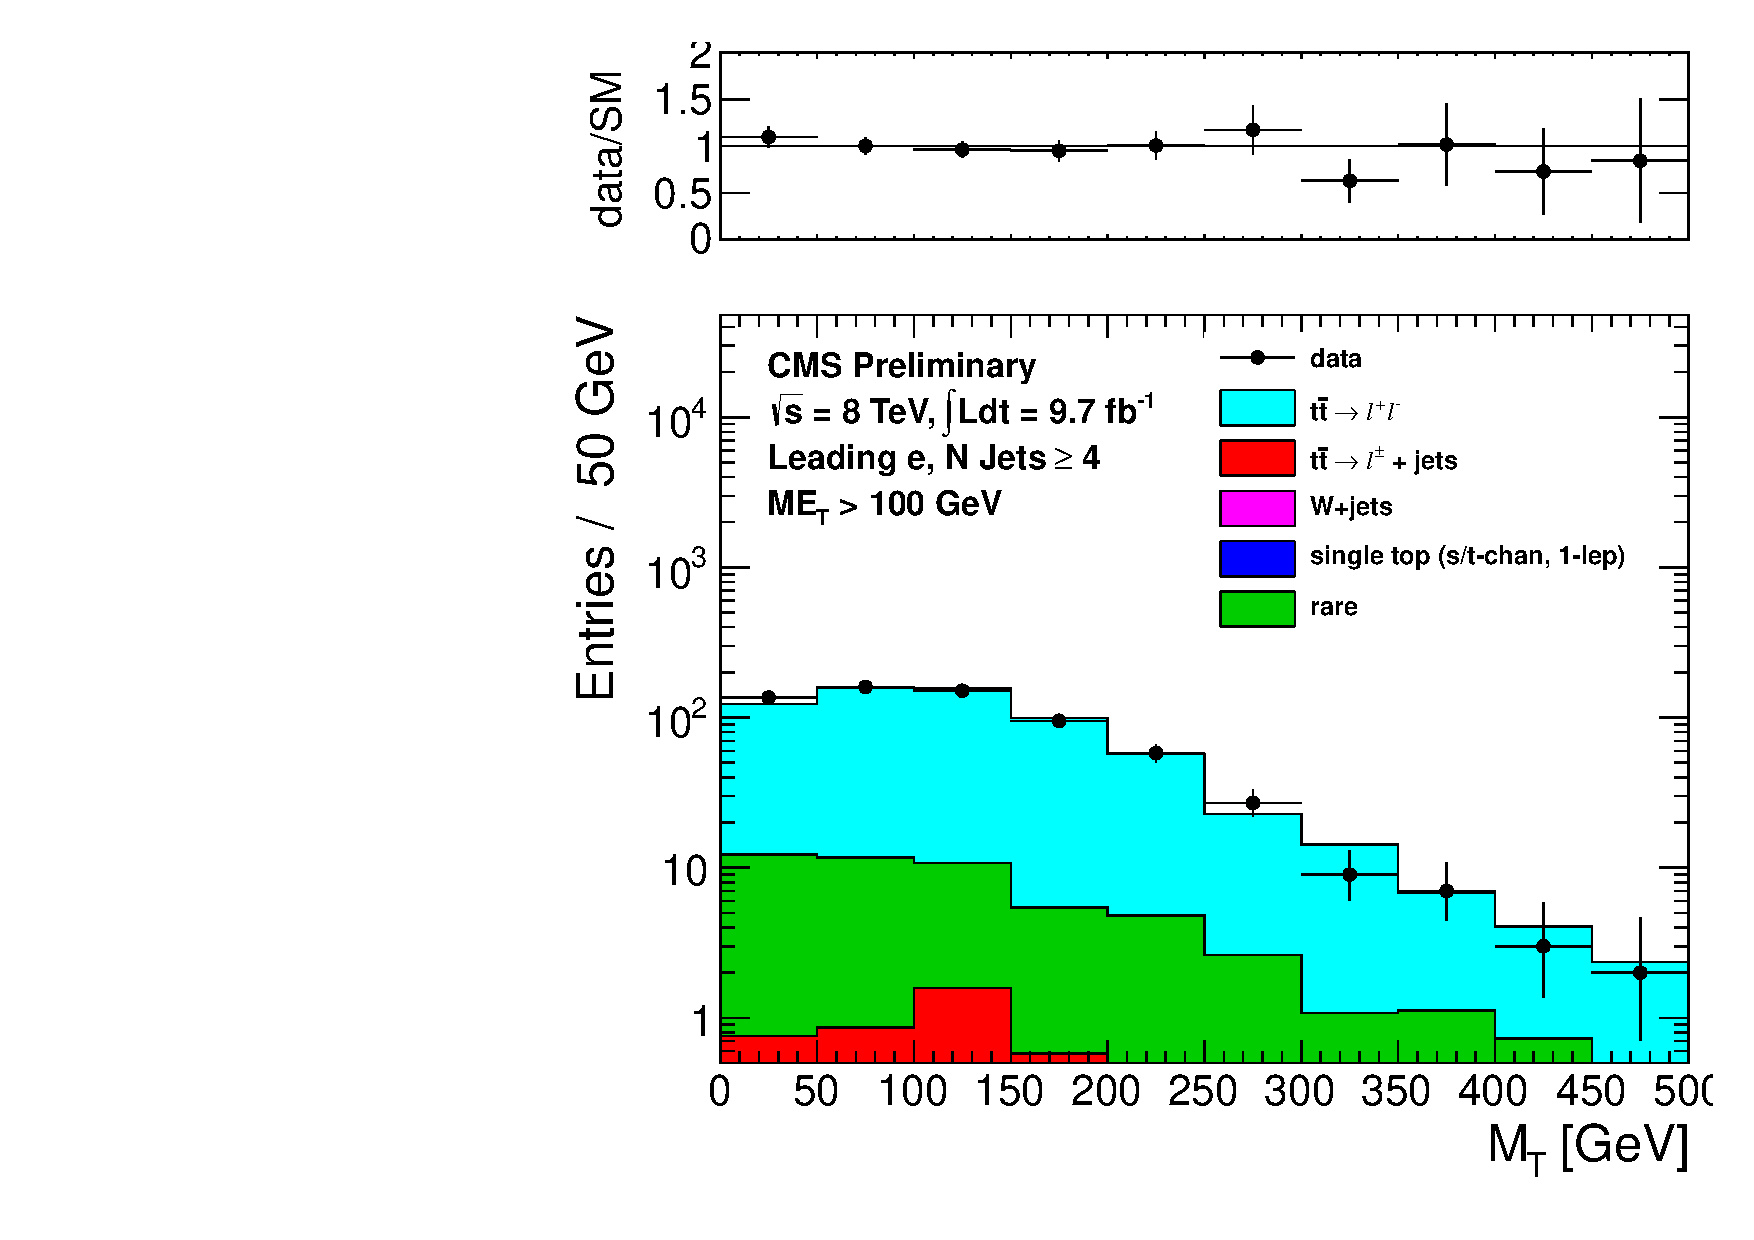
\includegraphics[width=0.5\linewidth]{plots/CR4plots/mt_met100_leadele_nj4.pdf}
    \caption{
      Comparison of the \met\ (top) and \mt\ for $\met>100$ (bottom) distributions in data vs. MC for events
      with a leading muon (left) and leading electron (right)
      satisfying the requirements of CR4. 
\label{fig:cr4met} 
}  
      \end{center}
\end{figure}

\begin{figure}[hbt]
  \begin{center}
	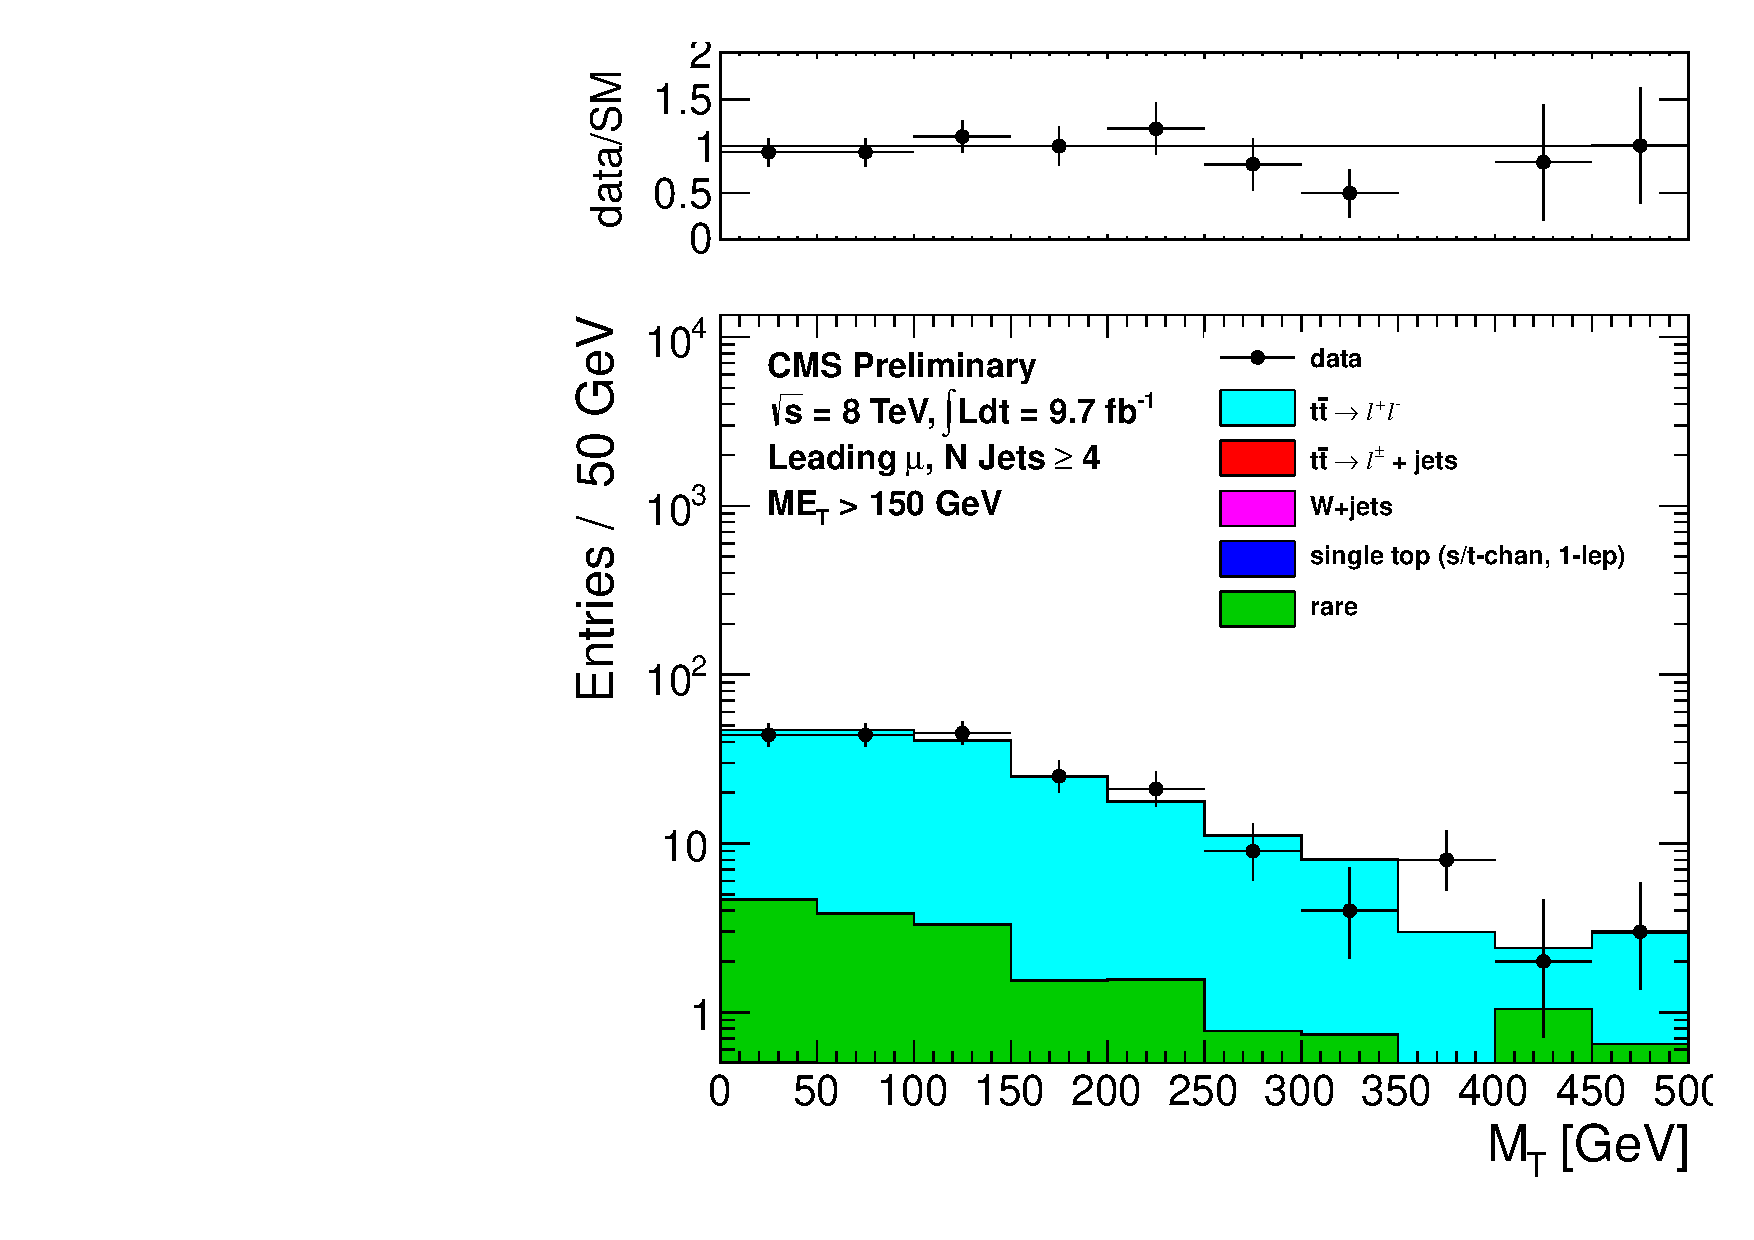
\includegraphics[width=0.5\linewidth]{plots/CR4plots/mt_met150_leadmuo_nj4.pdf}%
	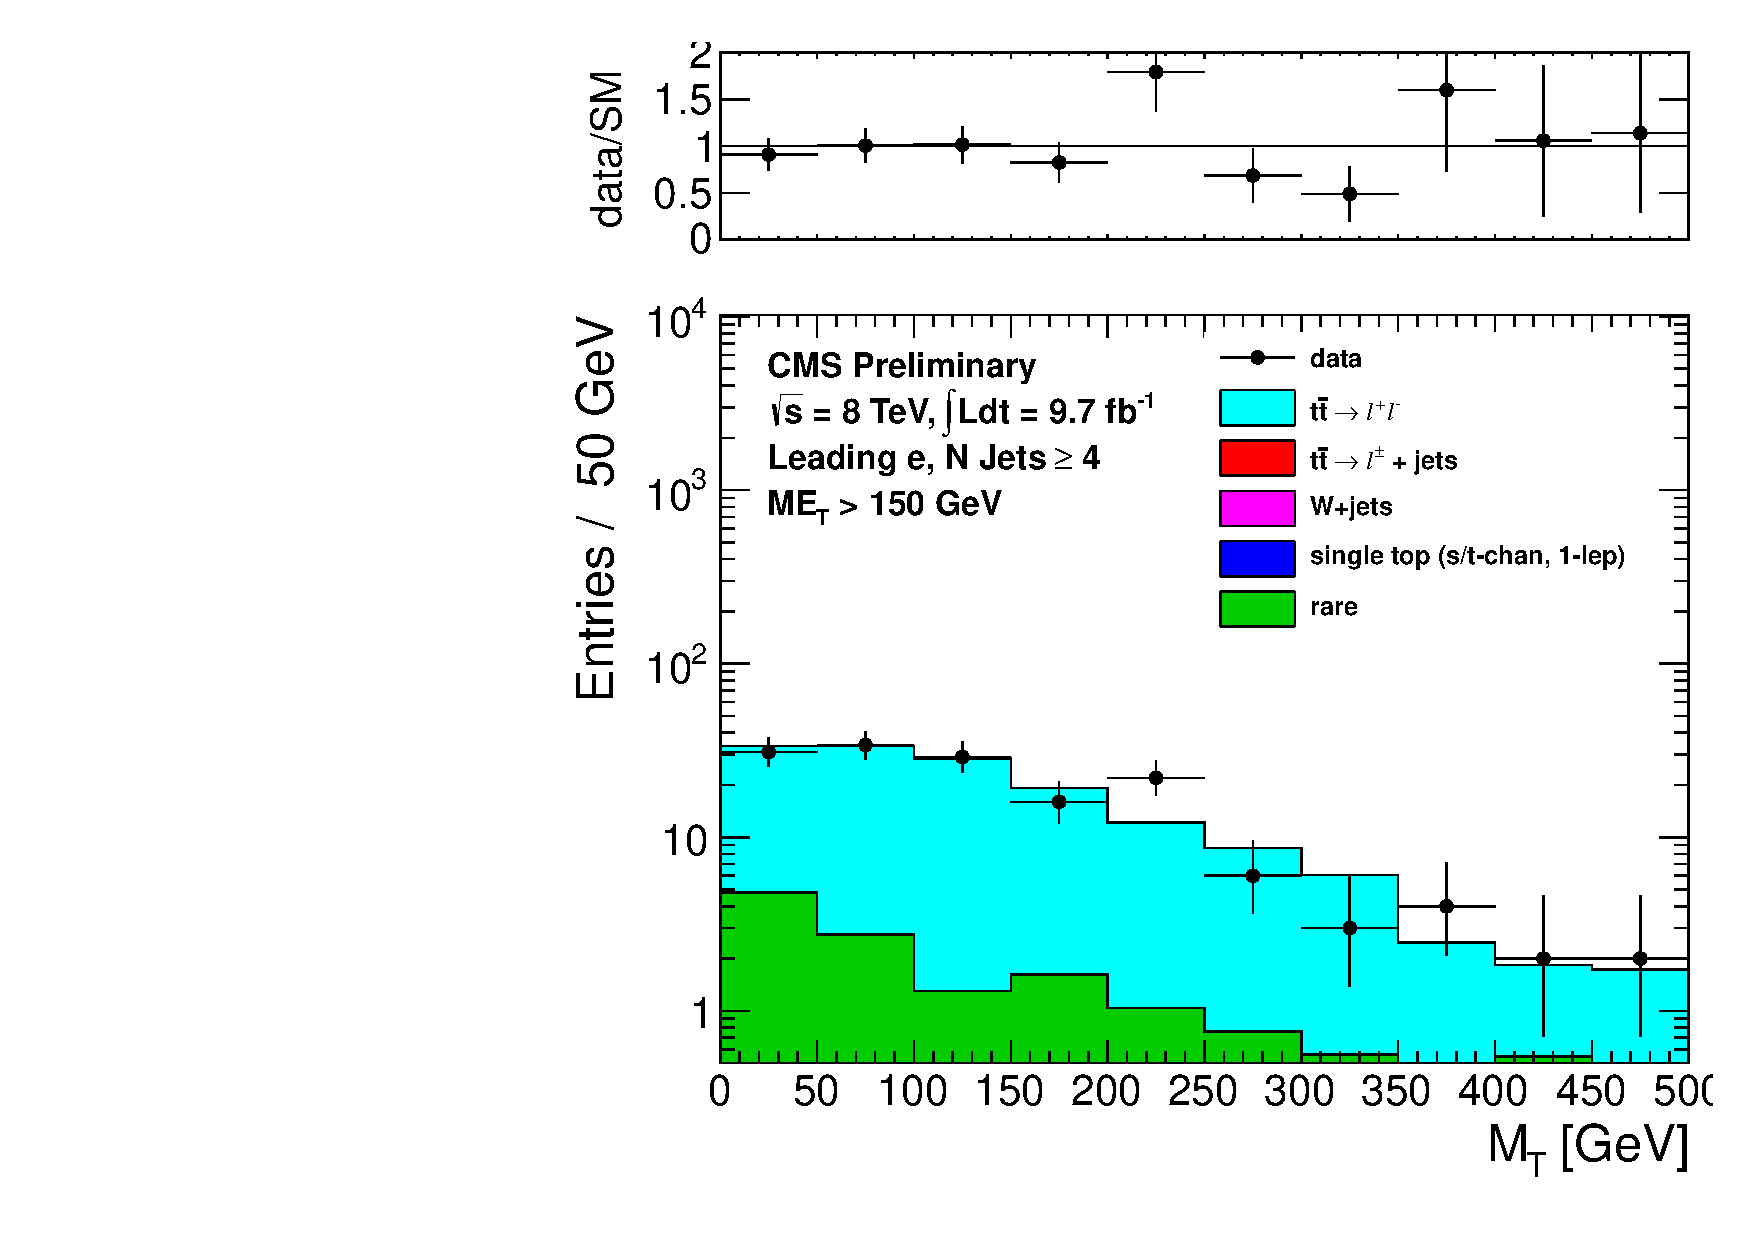
\includegraphics[width=0.5\linewidth]{plots/CR4plots/mt_met150_leadele_nj4.pdf}
	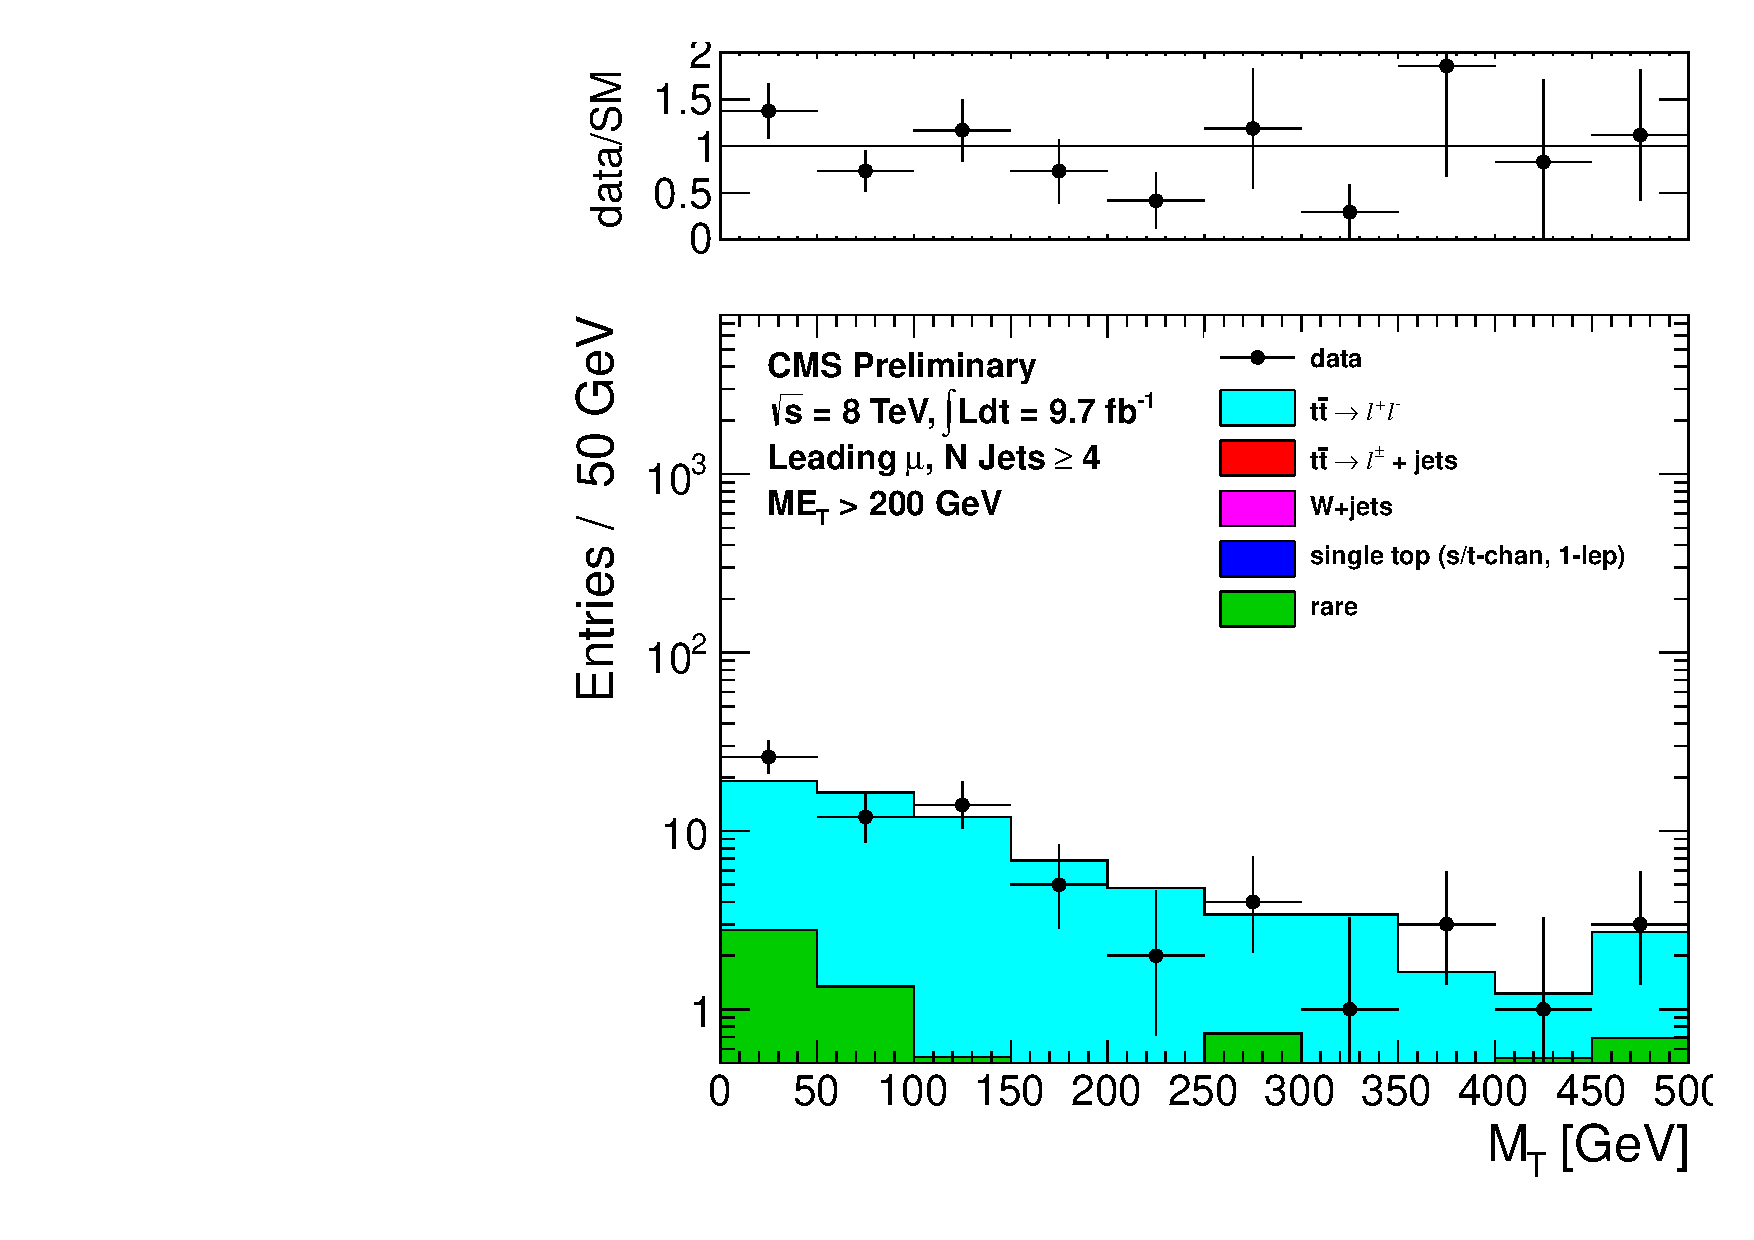
\includegraphics[width=0.5\linewidth]{plots/CR4plots/mt_met200_leadmuo_nj4.pdf}%
	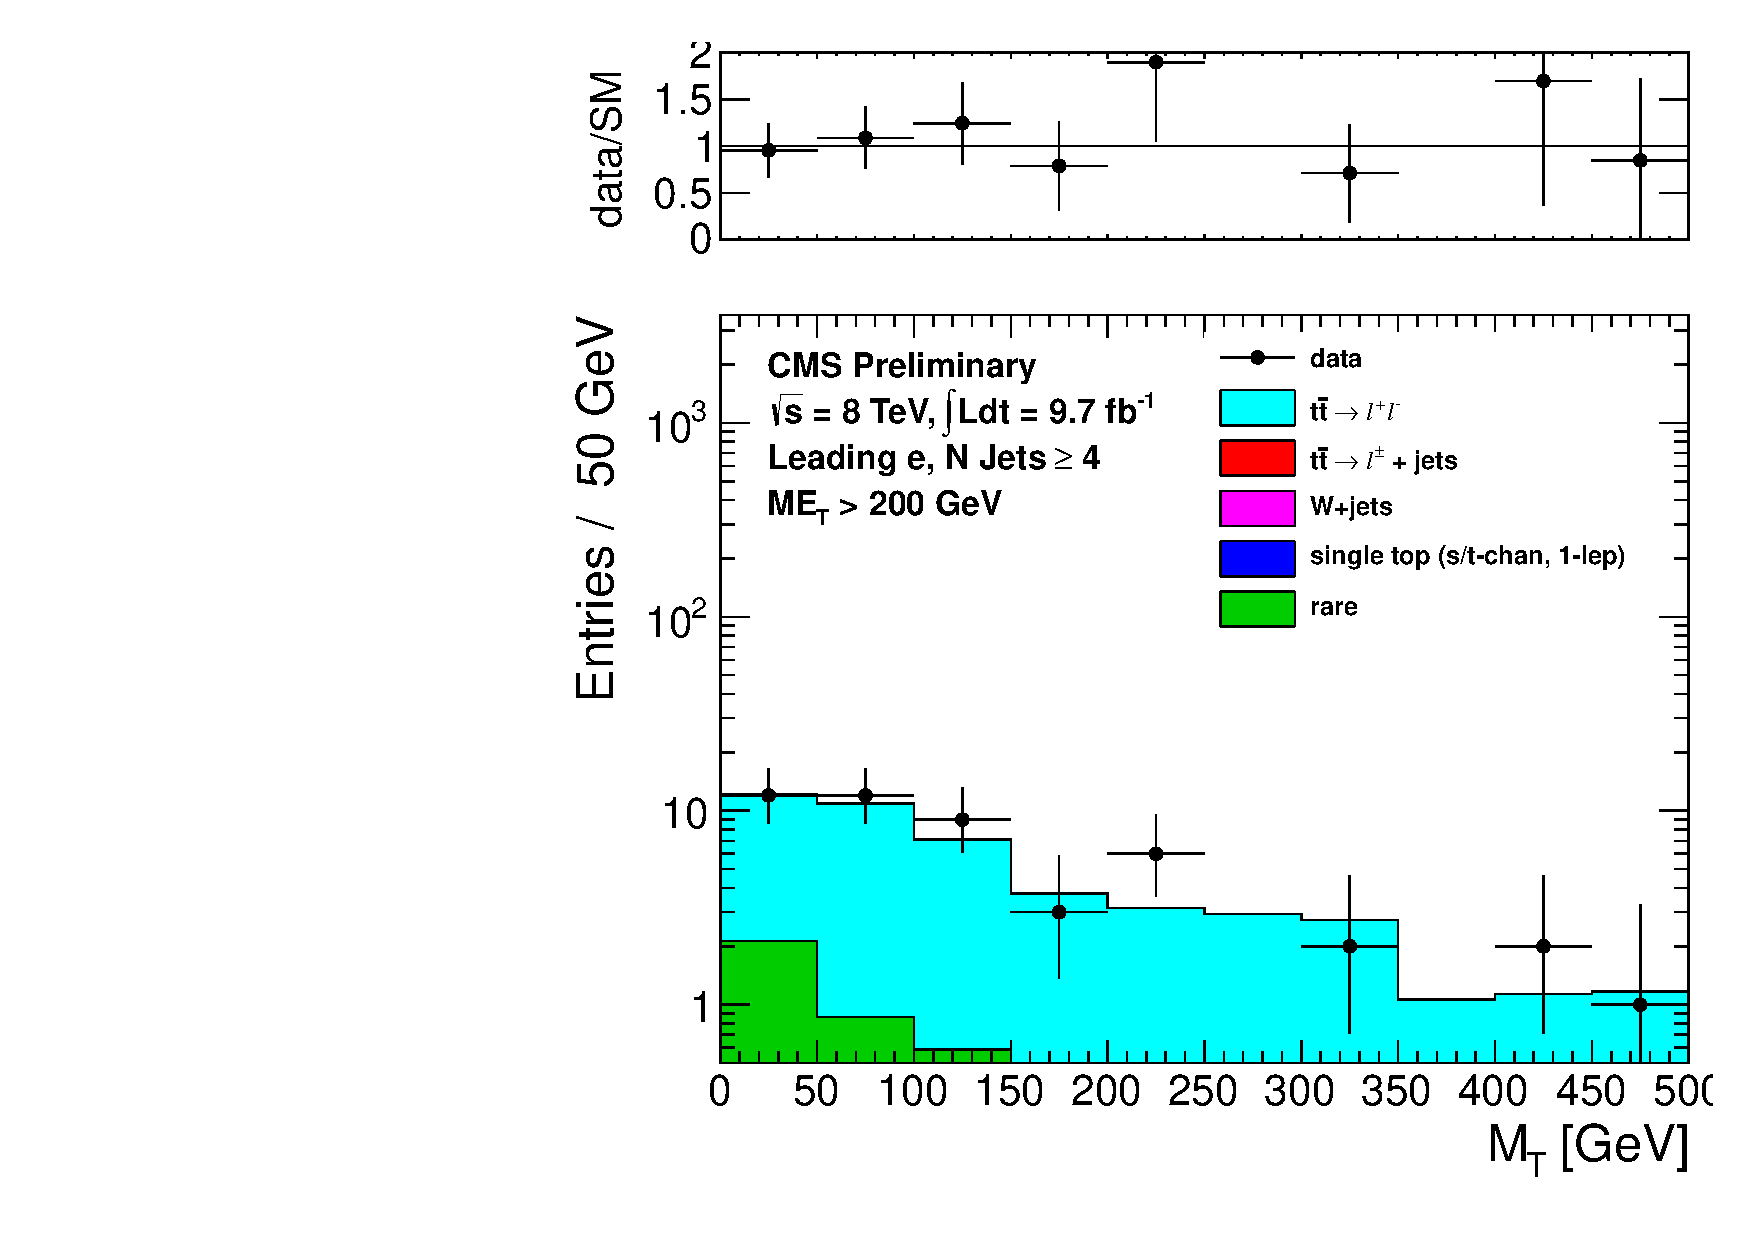
\includegraphics[width=0.5\linewidth]{plots/CR4plots/mt_met200_leadele_nj4.pdf}
	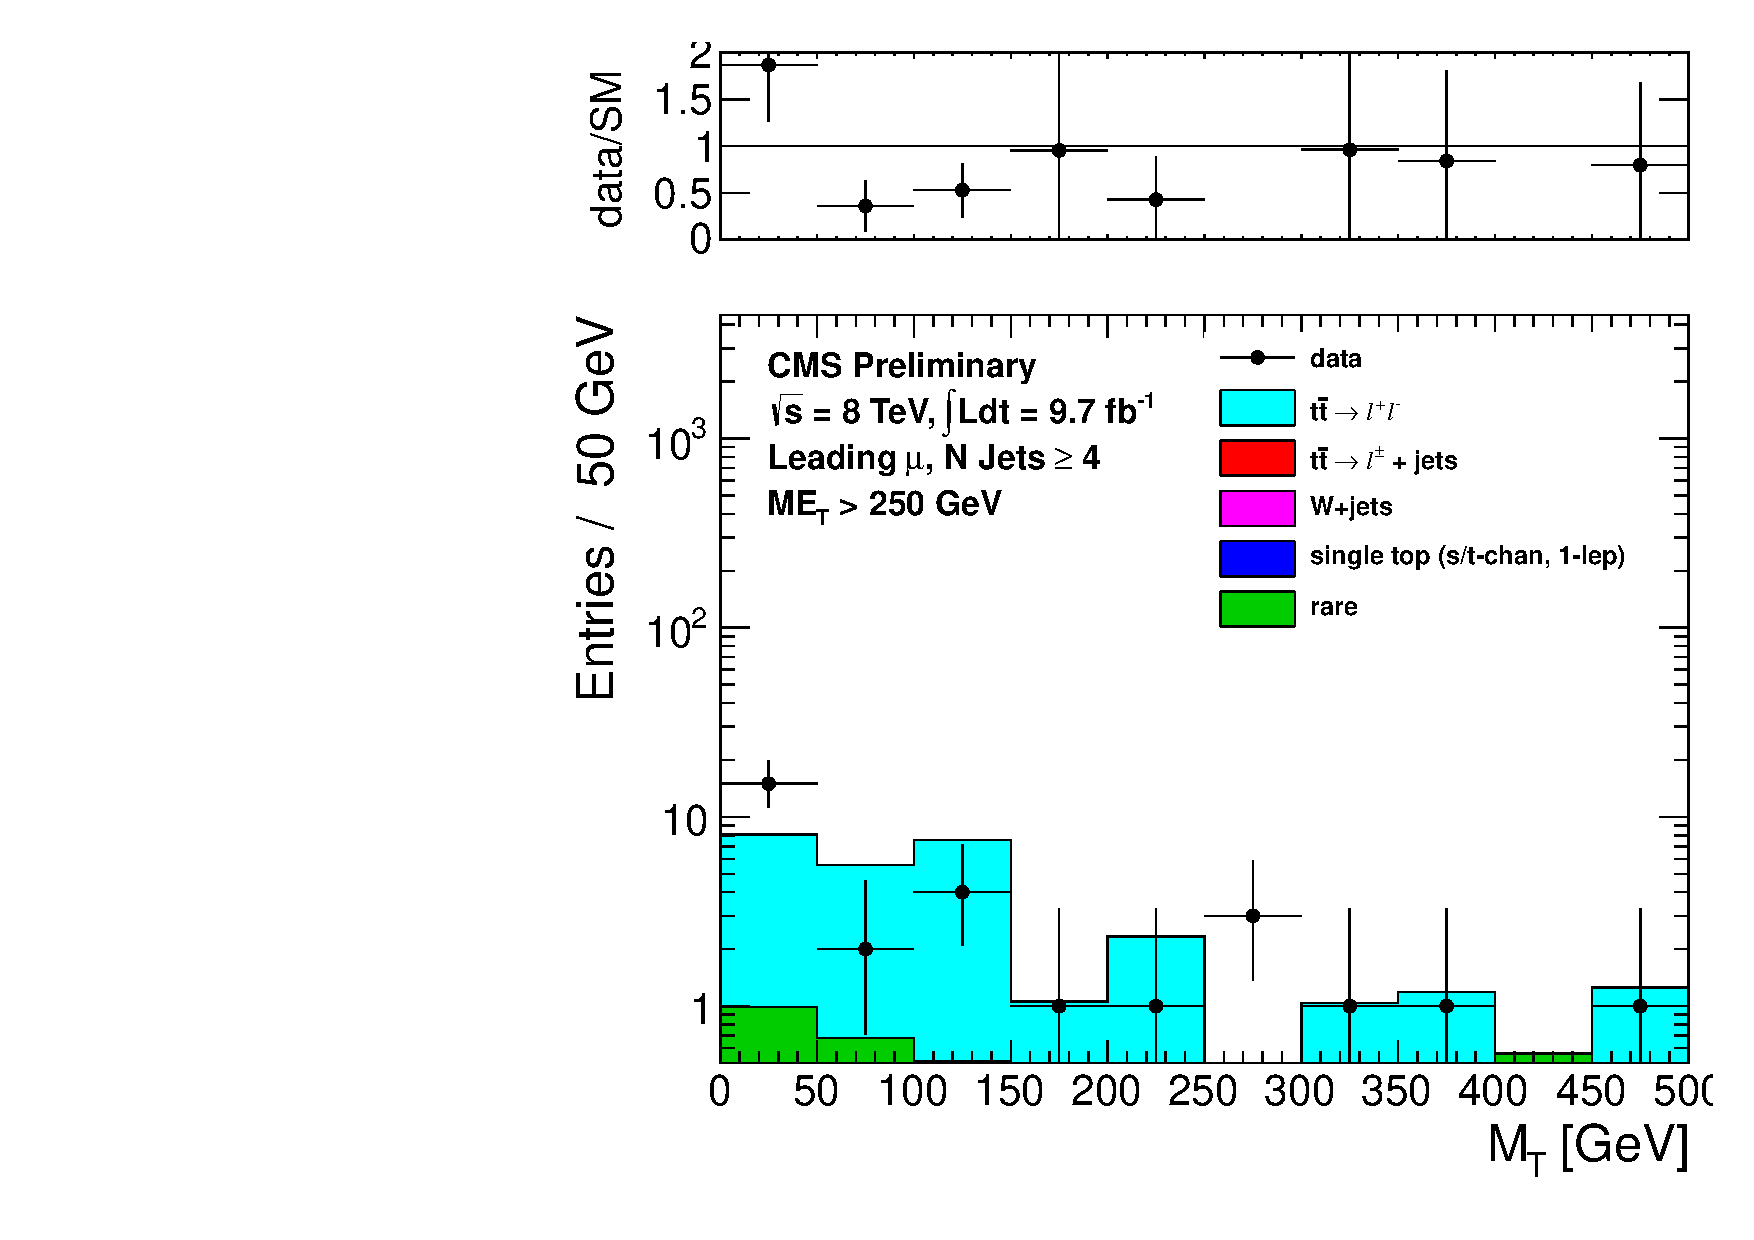
\includegraphics[width=0.5\linewidth]{plots/CR4plots/mt_met250_leadmuo_nj4.pdf}%
	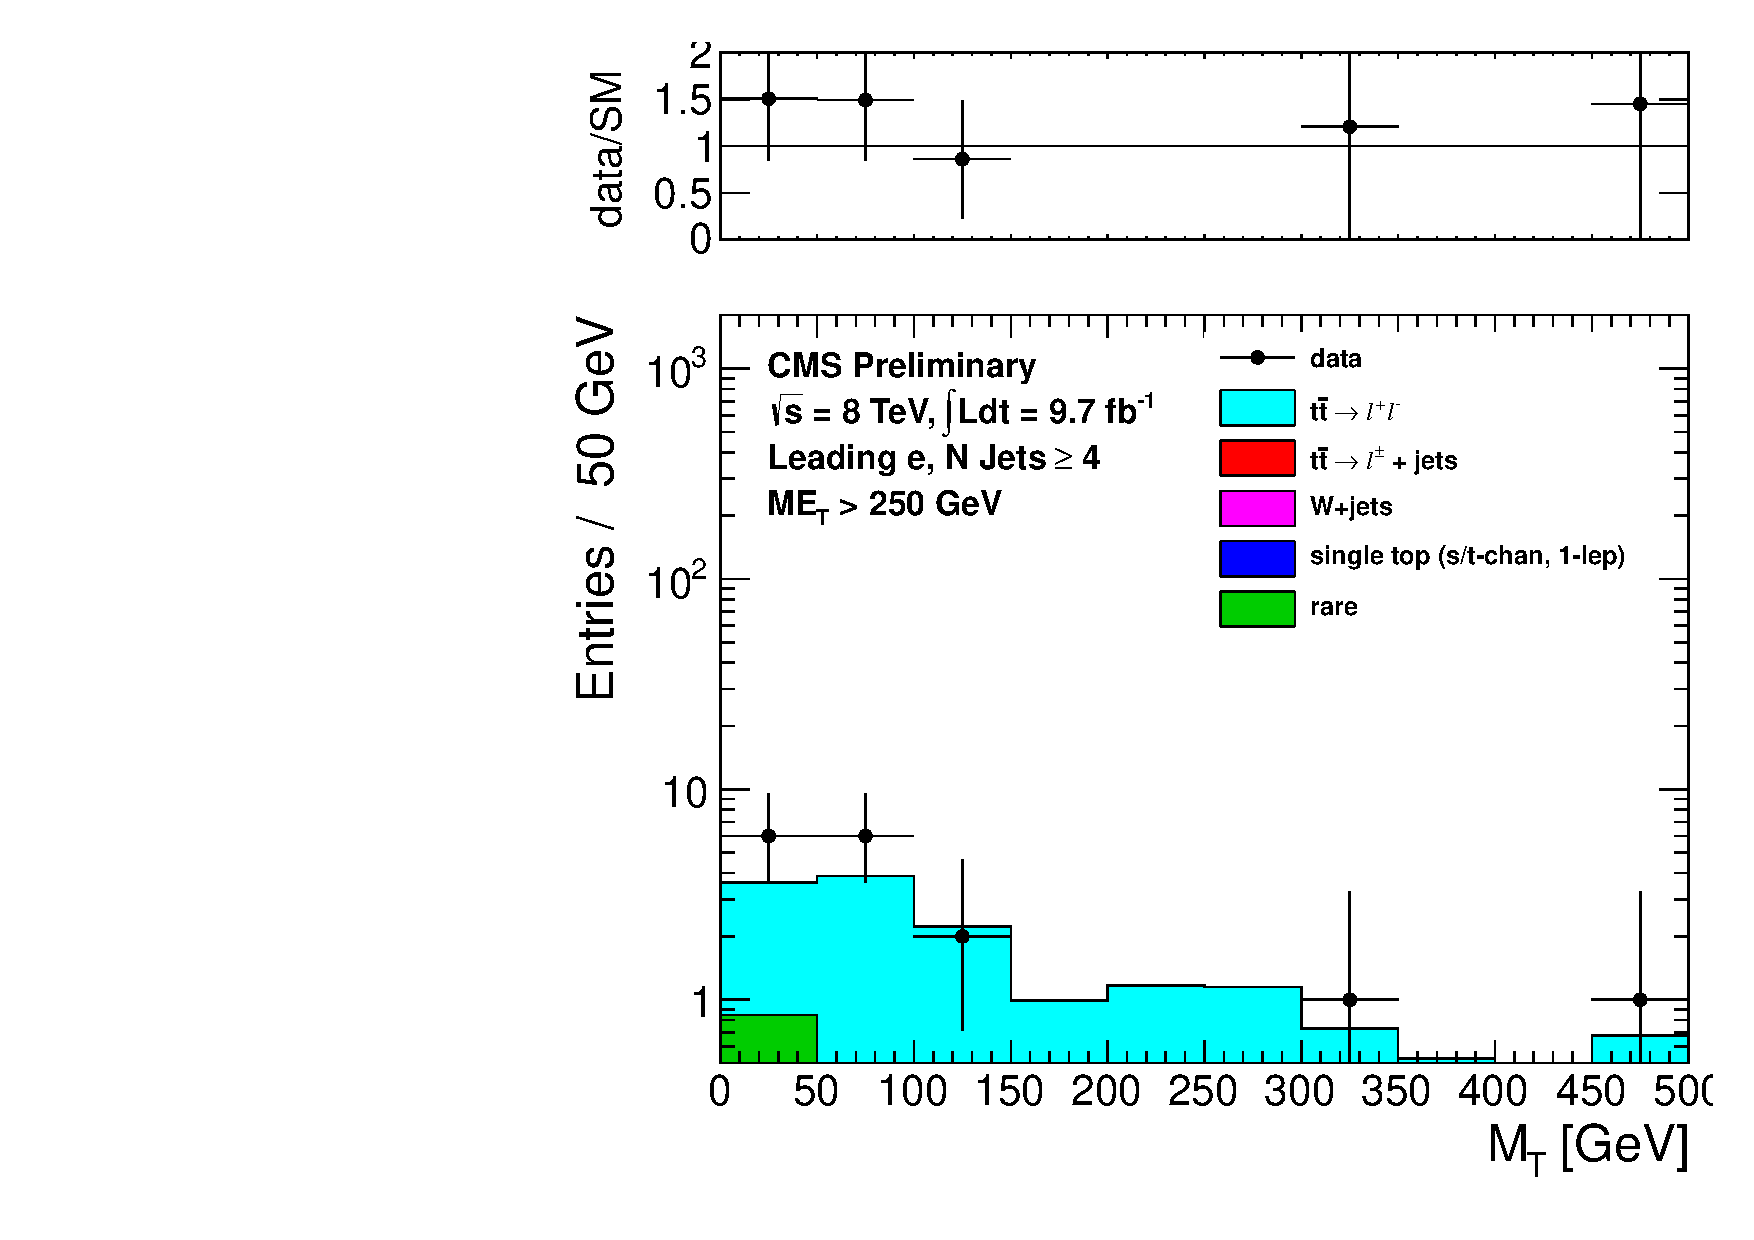
\includegraphics[width=0.5\linewidth]{plots/CR4plots/mt_met250_leadele_nj4.pdf}
    \caption{
      Comparison of the \mt\ distribution in data vs. MC for events
      with a leading muon (left) and leading electron (right)
      satisfying the requirements of CR4. The \met\ requirements used are
      150 GeV (top), 200 GeV (middle) and 250 GeV (bottom).
\label{fig:cr4mtrest} 
}  
      \end{center}
\end{figure}


\clearpage

\subsubsection{Validation of the lepton + isolated track Sample Prediction}

[EXPLAIN ALL THE CHECKS FOR CR5: LEPTON + ISOLATED TRACK SAMPLE]

[ALSO NEED BETTER TITLE FOR THIS SECTION!]

\begin{table}[!h]
\begin{center}
\begin{tabular}{l||c|c|c|c}
\hline
Sample              & CR5A & CR5B & CR5C & CR5D \\
\hline
\hline
Muon pre-veto \mt-SF 	  & $0.98 \pm 0.02$ & $0.95 \pm 0.04$ & $0.99 \pm 0.08$ & $0.89 \pm 0.15$ \\
Muon post-veto \mt-SF 	  & $1.28 \pm 0.07$ & $1.20 \pm 0.13$ & $1.22 \pm 0.24$ & $1.25 \pm 0.43$ \\
\hline
\hline
Electron pre-veto \mt-SF 	  & $0.83 \pm 0.02$ & $0.75 \pm 0.04$ & $0.64 \pm 0.07$ & $0.63 \pm 0.12$ \\
Electron post-veto \mt-SF 	  & $1.10 \pm 0.08$ & $1.02 \pm 0.11$ & $0.89 \pm 0.19$ & $1.27 \pm 0.41$ \\
\hline
\end{tabular}
\caption{ \mt\ peak Data/MC scale factors. The pre-veto SFs are applied to the
  \ttdl\ sample, while the post-veto SFs are applied to the single
  lepton samples. The raw MC is used for backgrounds from rare processes.
  The uncertainties are statistical only.
\label{tab:cr5mtsf}}
\end{center}
\end{table}


\begin{table}[!h]
\begin{center}
\begin{tabular}{l||c|c|c|c}
\hline
Sample              & CR5A & CR5B & CR5C & CR5D \\
\hline
\hline
Muon MC 		  & $293 \pm 9$ & $161 \pm 7$ & $51 \pm 4$ & $16 \pm 2$ \\
Muon Data 		  & $315$ & $165$ & $62$ & $13$ \\
\hline
Muon Data/MC SF 	  & $1.07 \pm 0.07$ & $1.03 \pm 0.09$ & $1.21 \pm 0.18$ & $0.82 \pm 0.25$ \\
\hline
\hline
Electron MC 		  & $253 \pm 8$ & $126 \pm 5$ & $37 \pm 3$ & $12 \pm 2$ \\
Electron Data 		  & $286$ & $135$ & $39$ & $15$ \\
\hline
Electron Data/MC SF 	  & $1.13 \pm 0.08$ & $1.07 \pm 0.10$ & $1.07 \pm 0.19$ & $1.21 \pm 0.35$ \\
\hline
\end{tabular}
\caption{ Yields in \mt\ tail comparing the MC prediction (after
  applying SFs) to data. The uncertainties are statistical only.
\label{tab:cr5yields}}
\end{center}
\end{table}

\begin{figure}[hbt]
  \begin{center}
	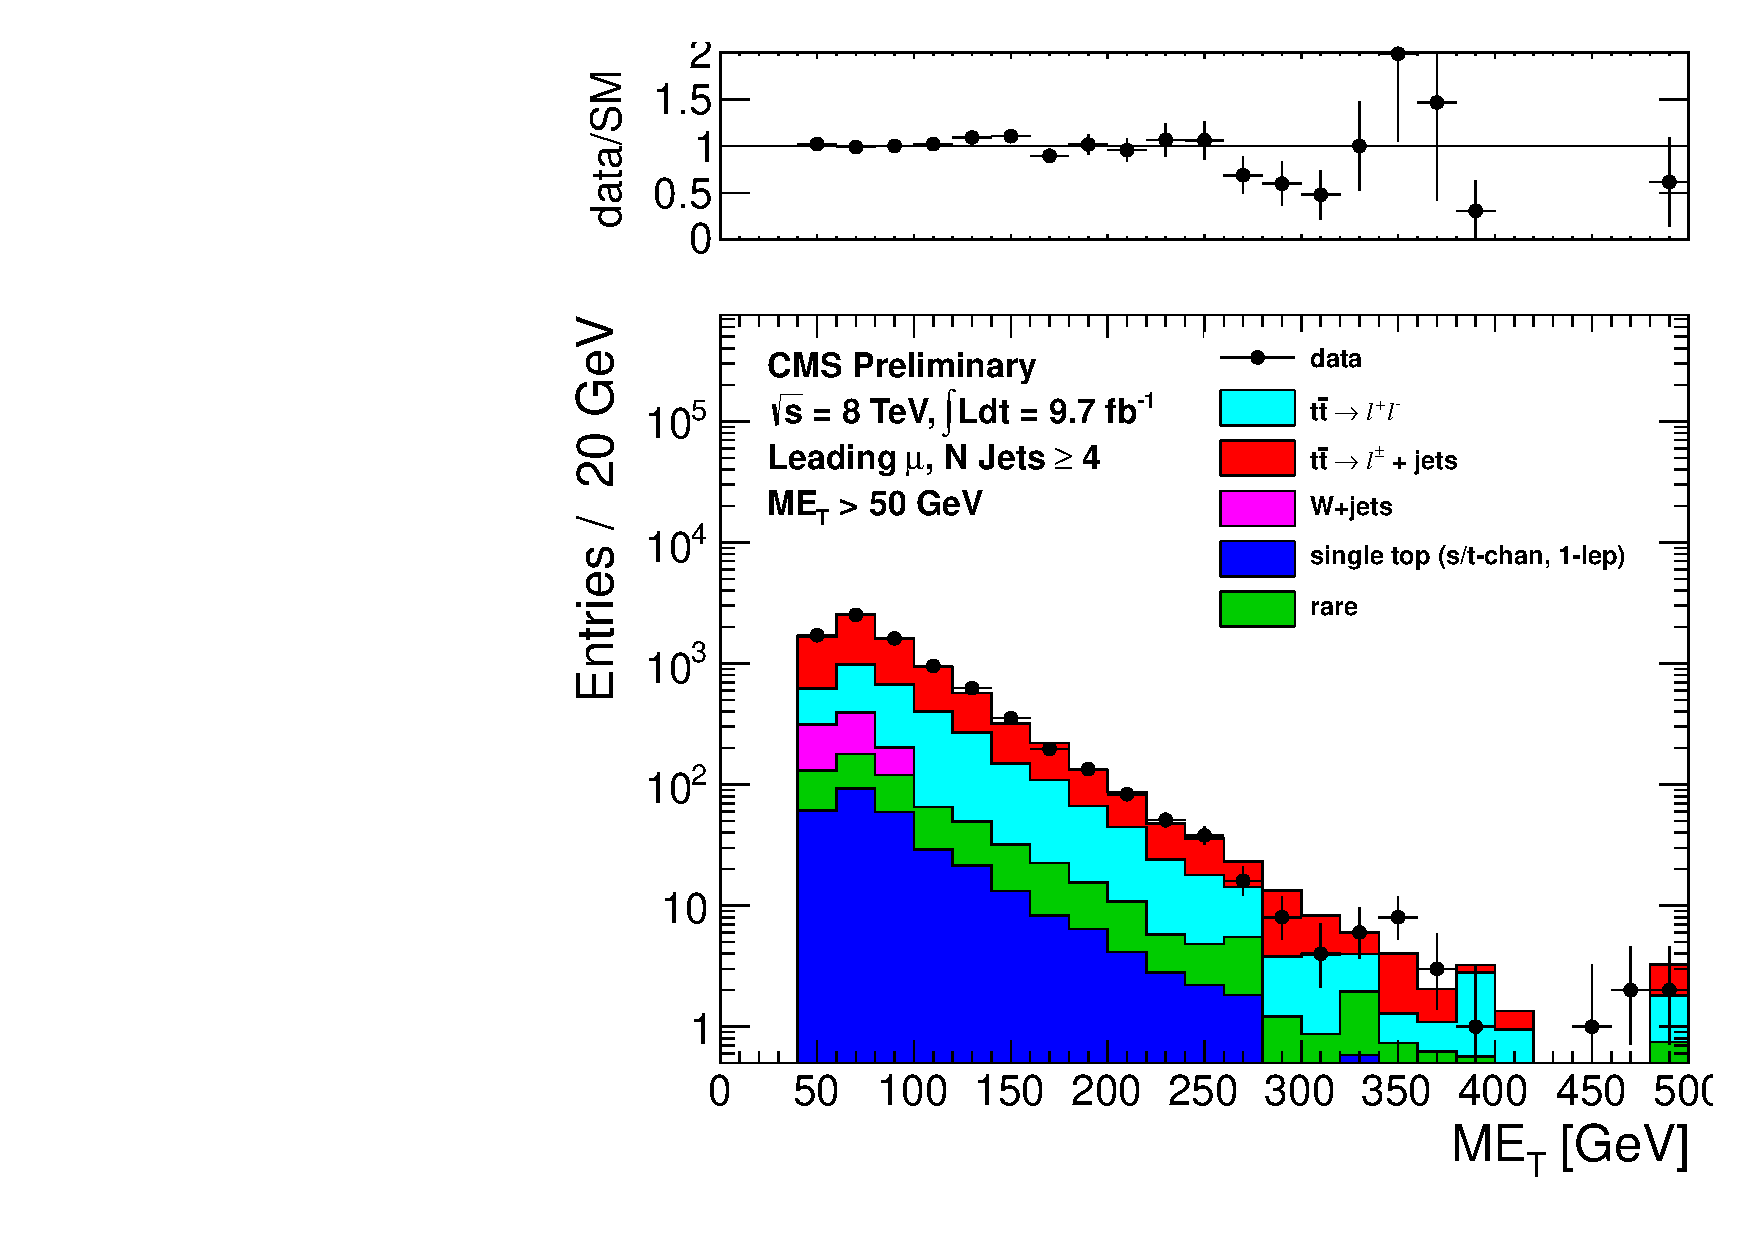
\includegraphics[width=0.5\linewidth]{plots/CR5plots/met_met50_leadmuo_nj4.pdf}%
	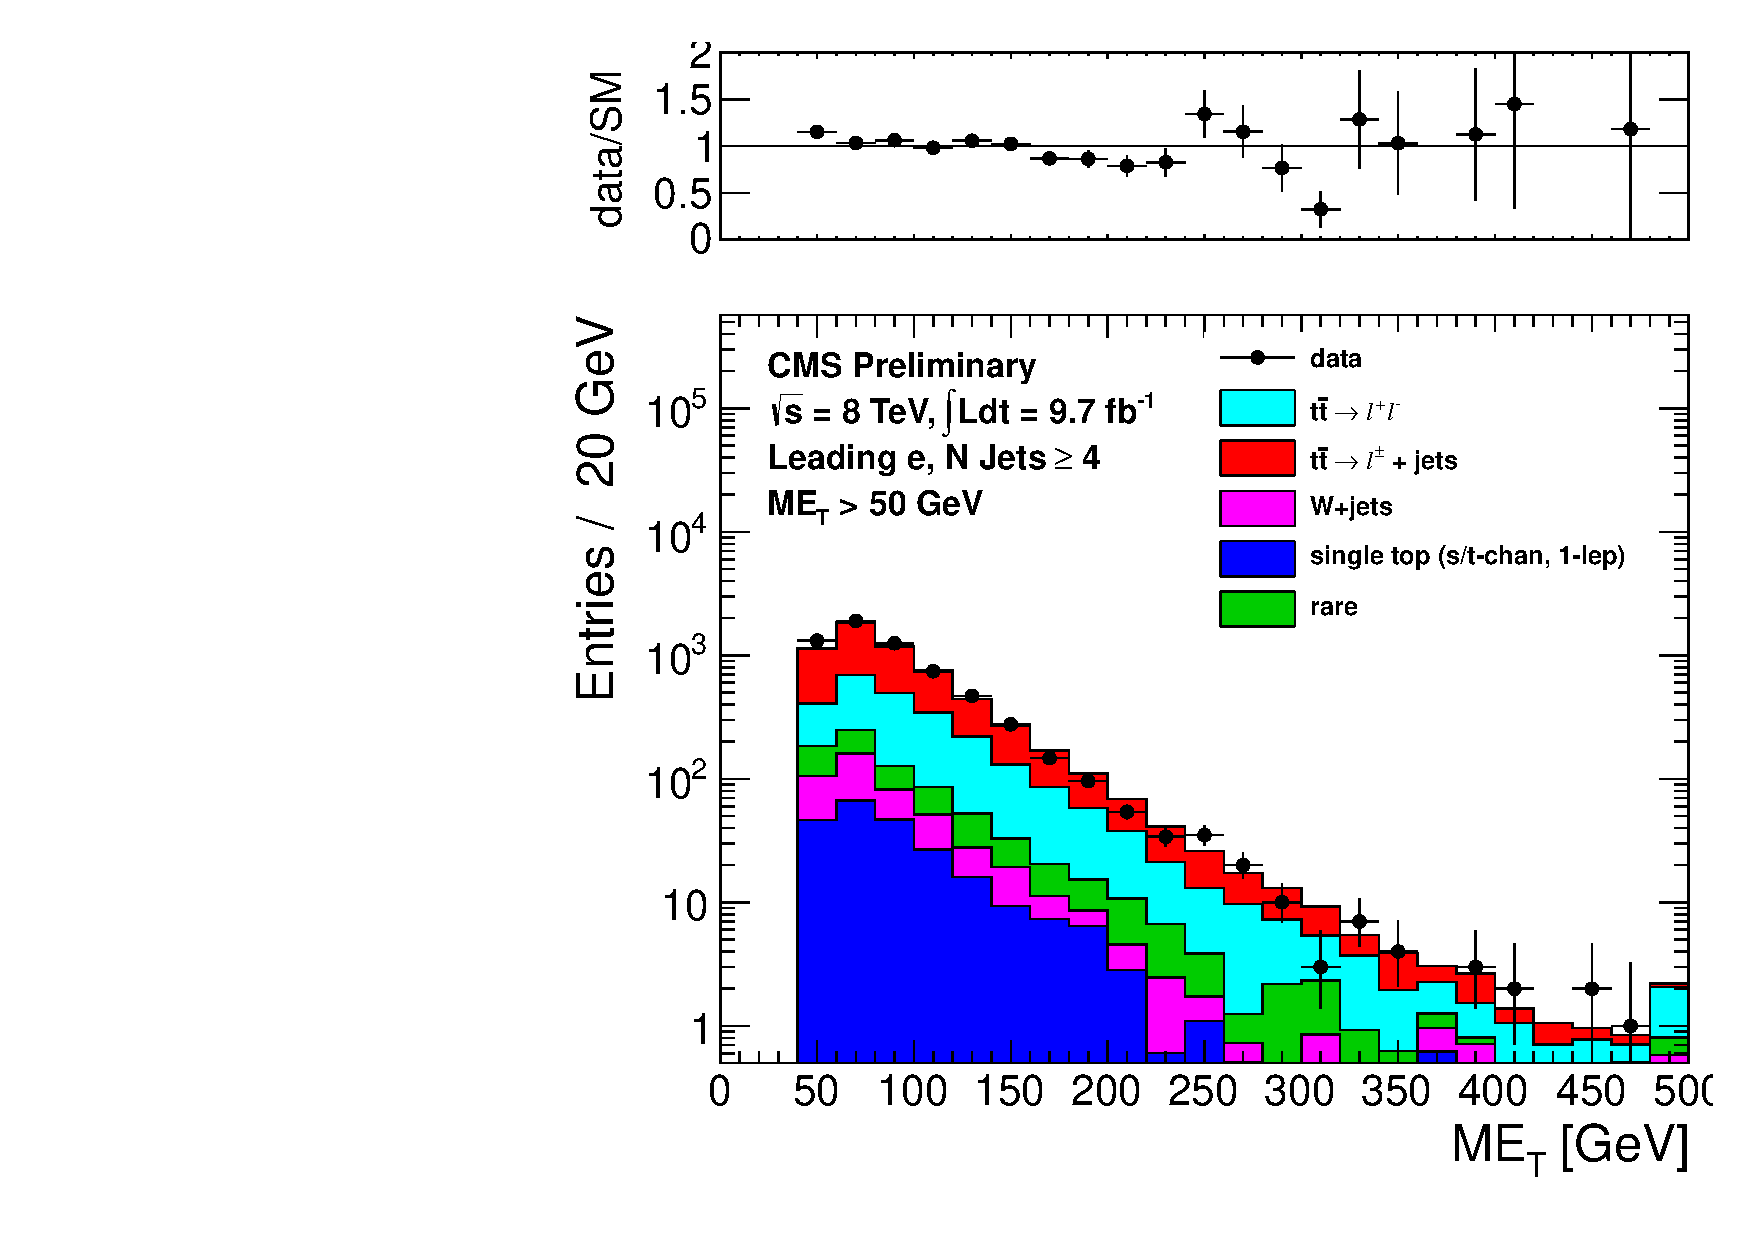
\includegraphics[width=0.5\linewidth]{plots/CR5plots/met_met50_leadele_nj4.pdf}
	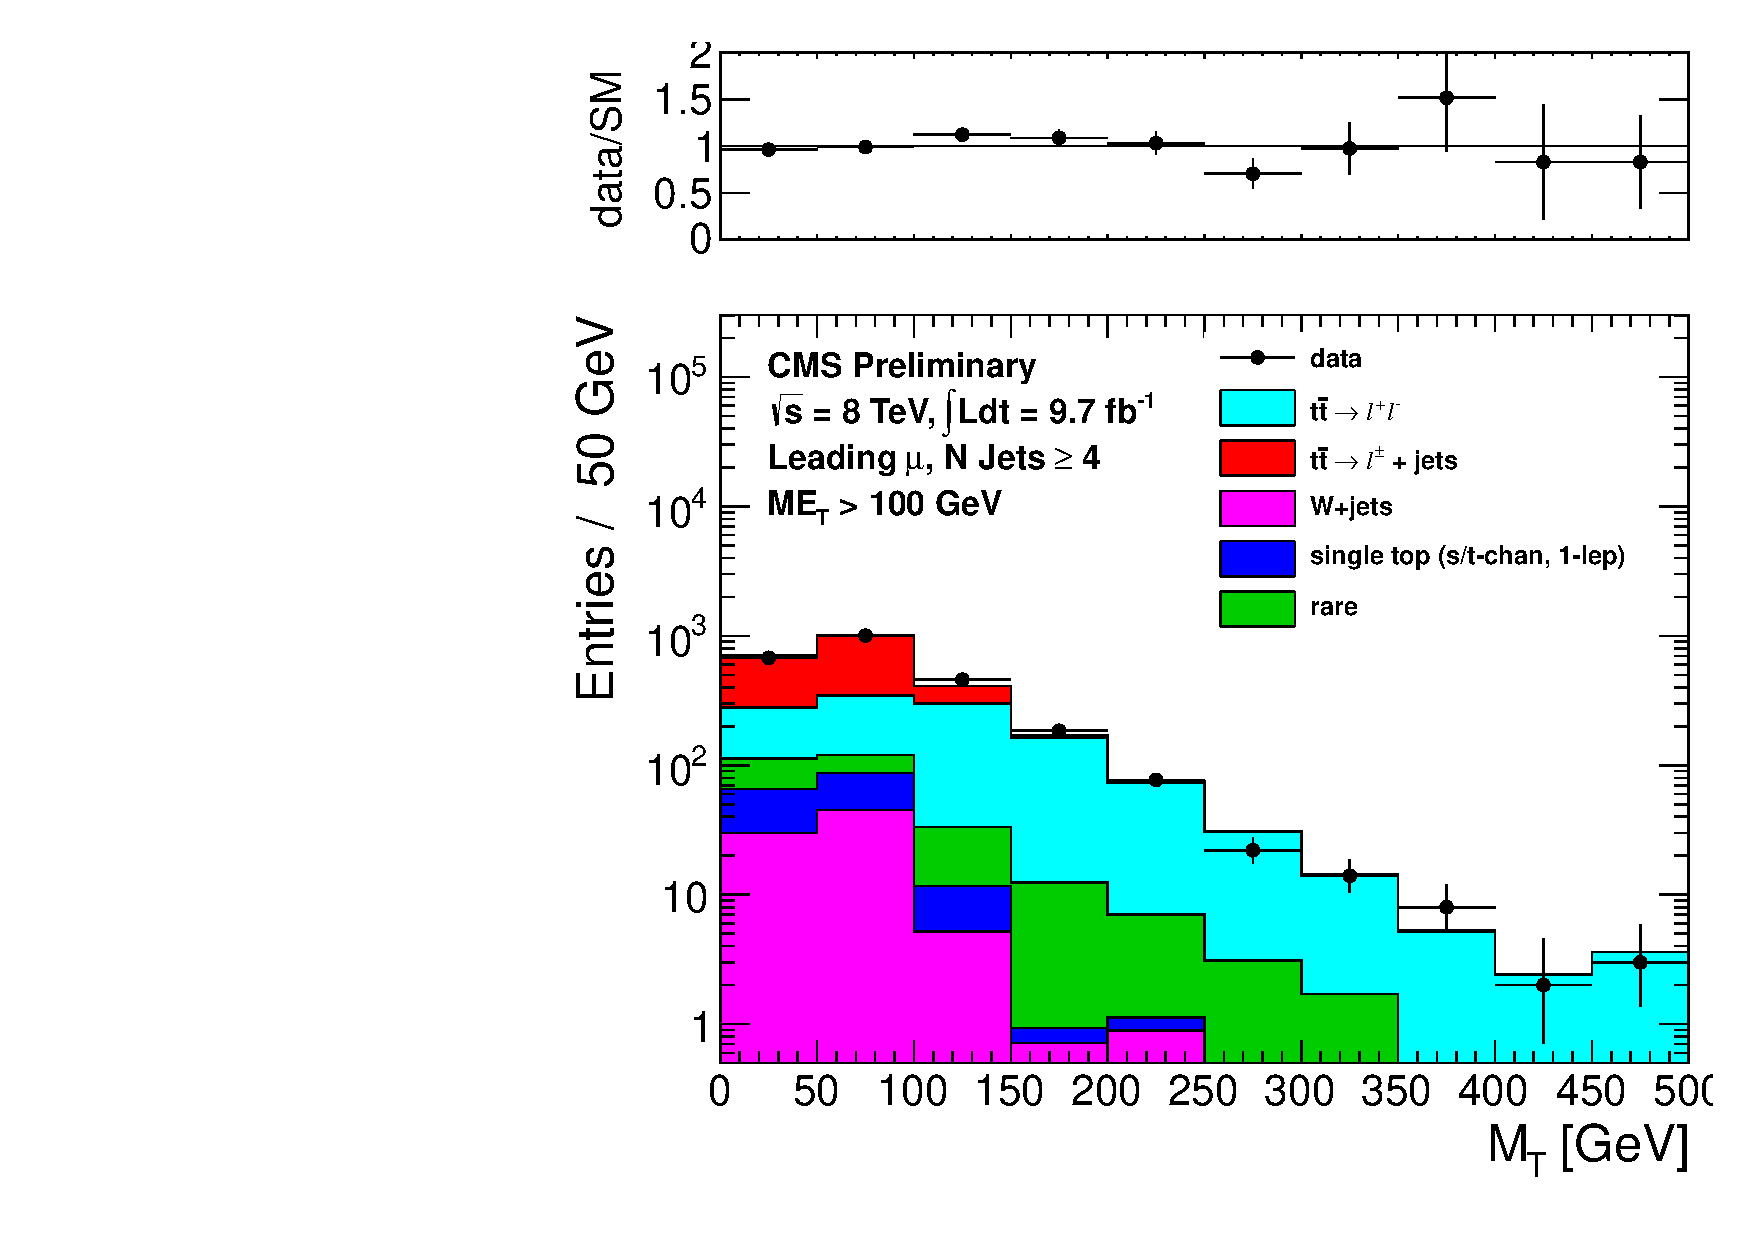
\includegraphics[width=0.5\linewidth]{plots/CR5plots/mt_met100_leadmuo_nj4.pdf}%
	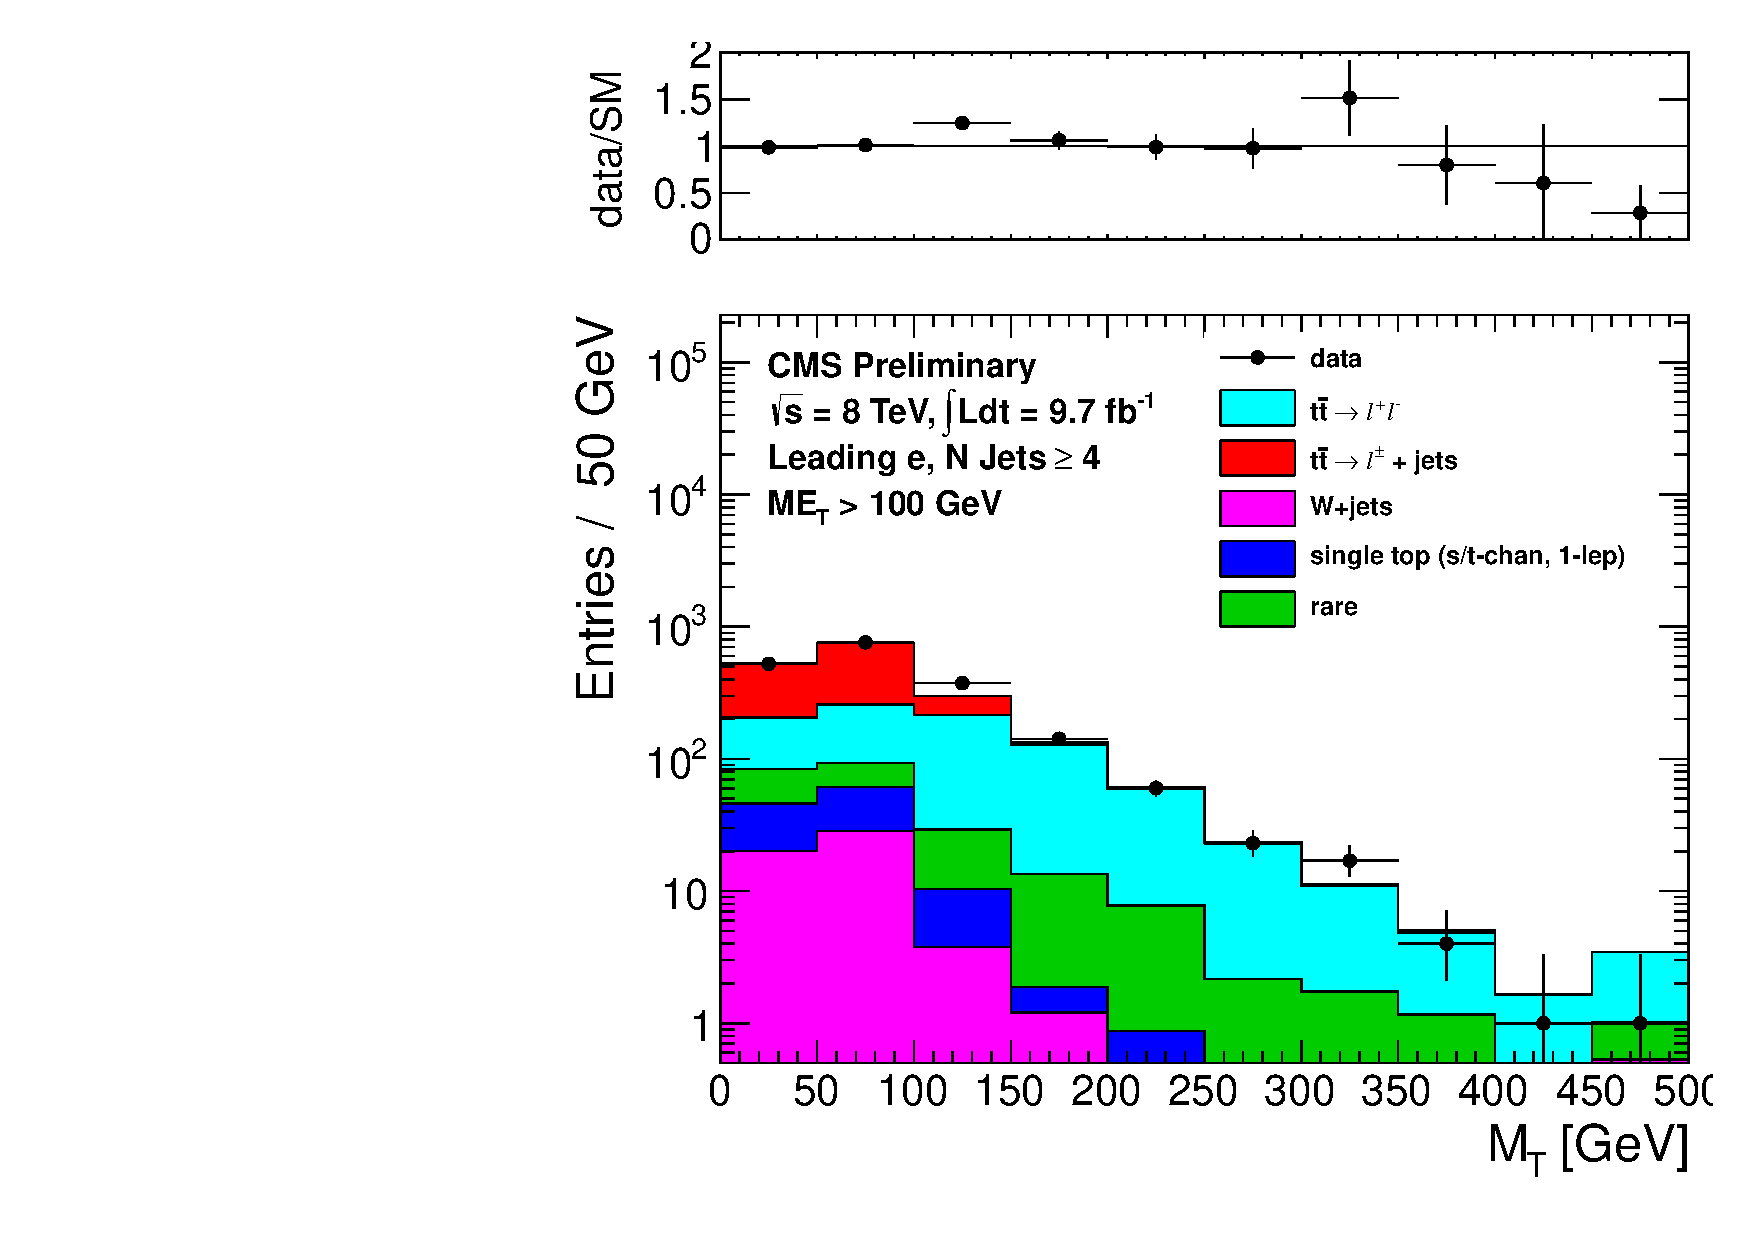
\includegraphics[width=0.5\linewidth]{plots/CR5plots/mt_met100_leadele_nj4.pdf}
    \caption{
      Comparison of the \met\ (top) and \mt\ for $\met>100$ (bottom) distributions in data vs. MC for events
      with a leading muon (left) and leading electron (right)
      satisfying the requirements of CR5. 
\label{fig:cr5met} 
}  
      \end{center}
\end{figure}

\begin{figure}[hbt]
  \begin{center}
	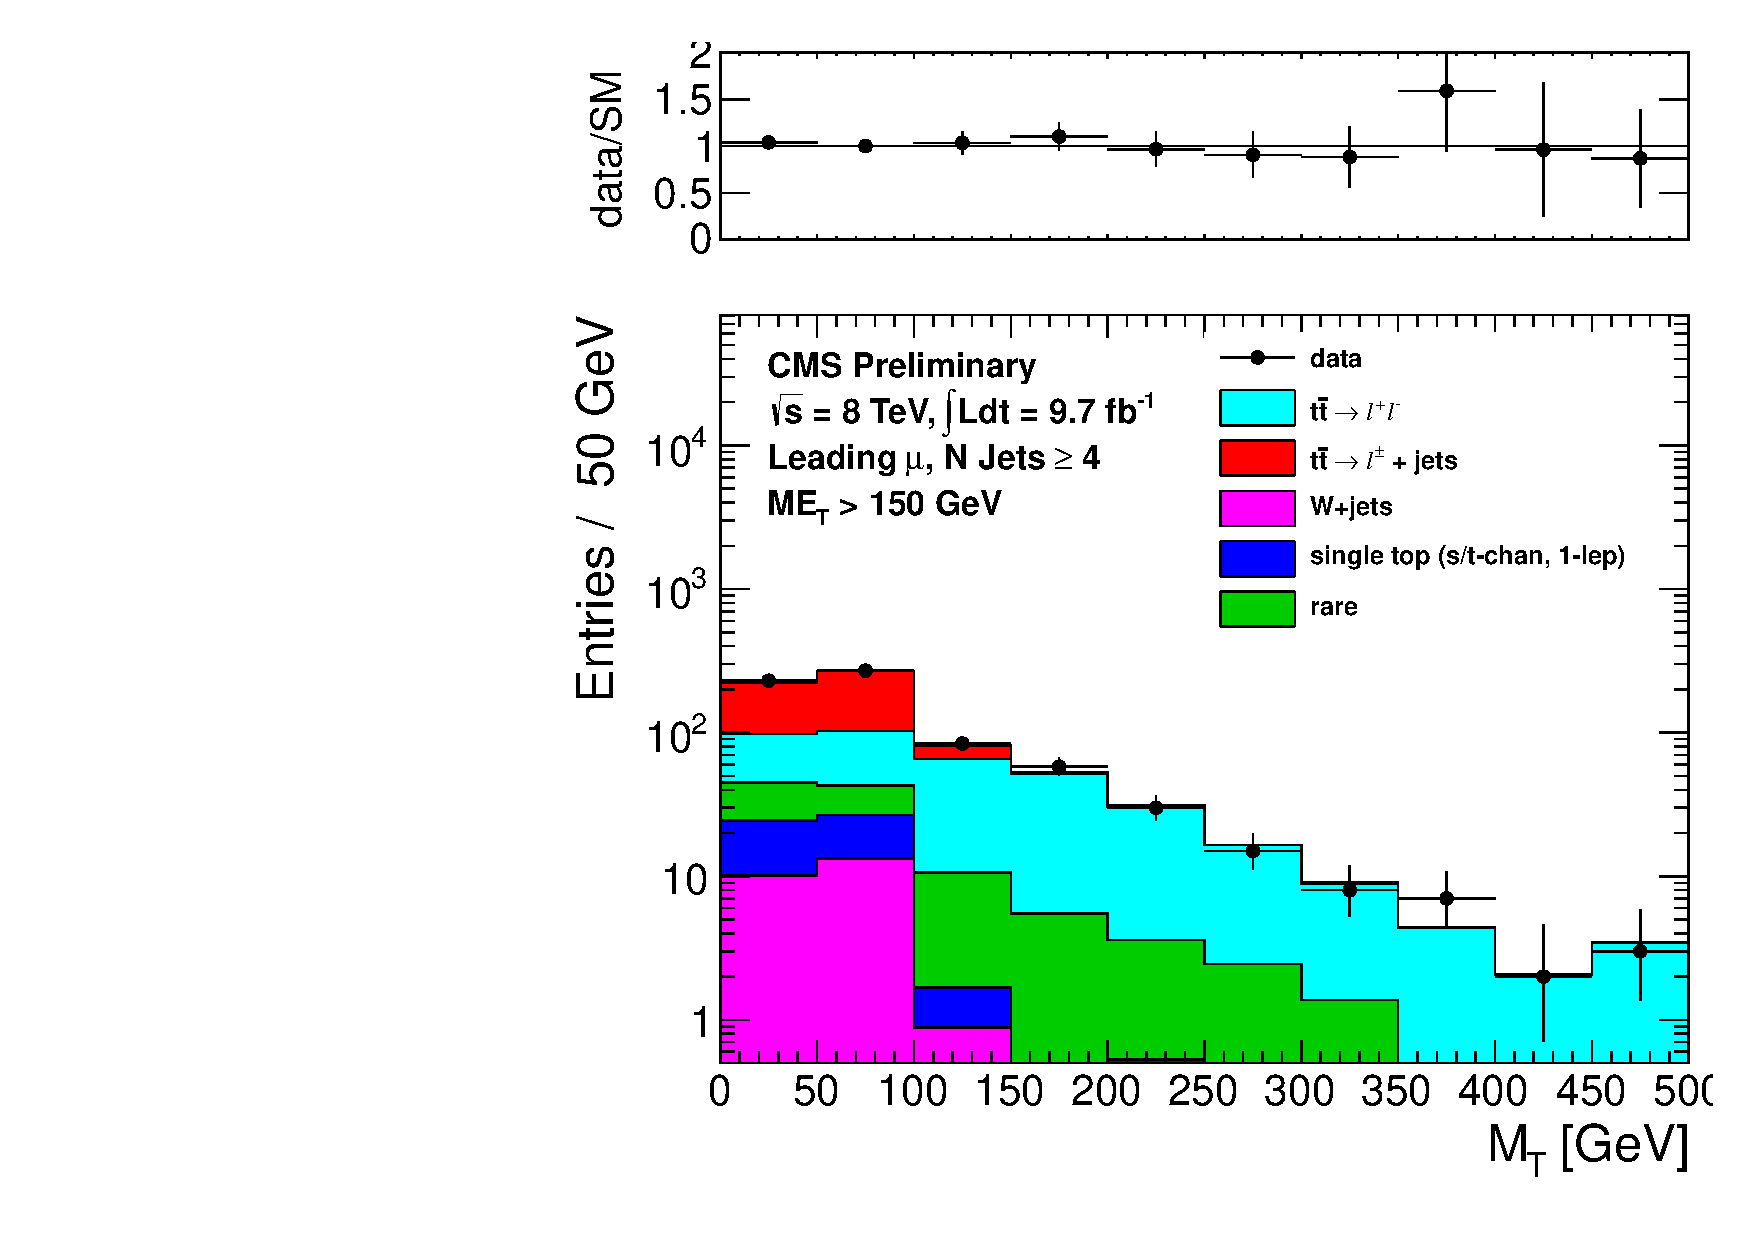
\includegraphics[width=0.5\linewidth]{plots/CR5plots/mt_met150_leadmuo_nj4.pdf}%
	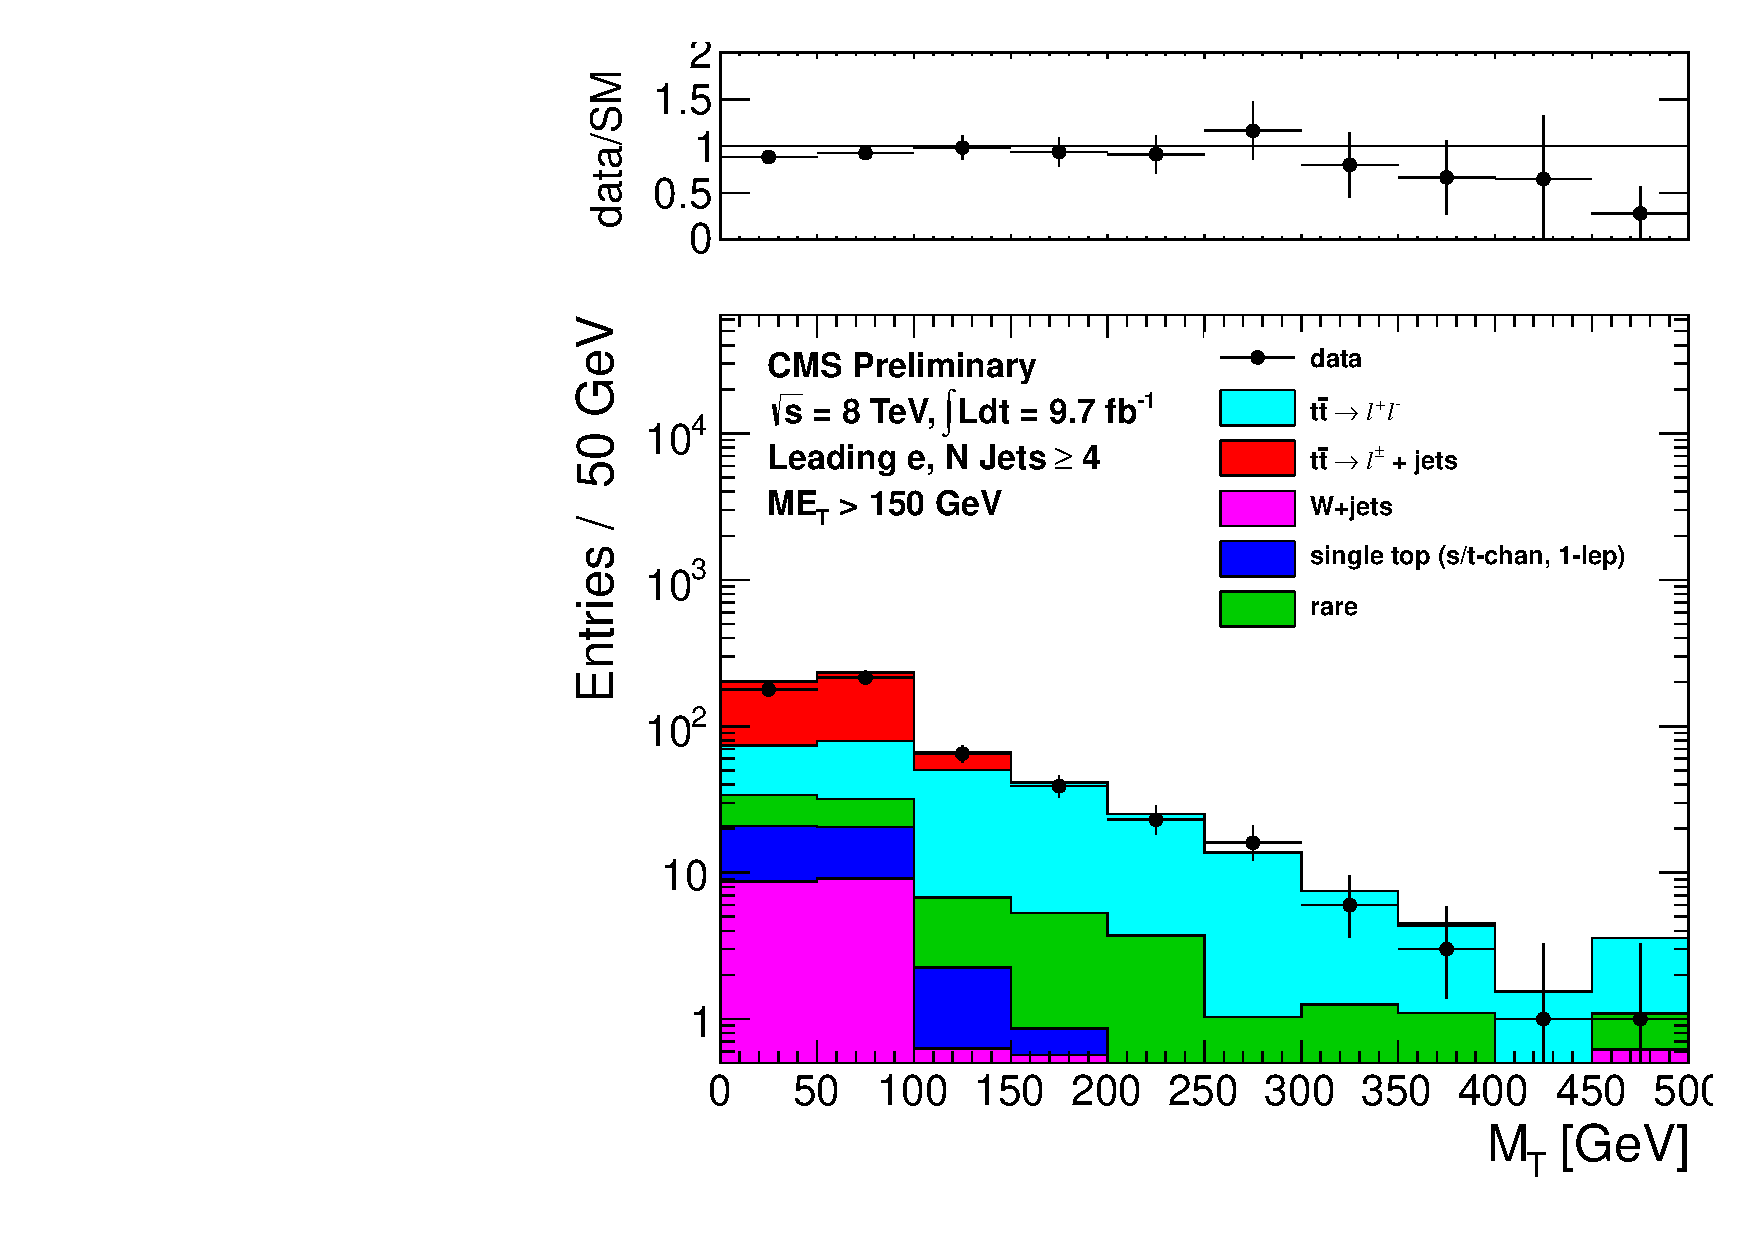
\includegraphics[width=0.5\linewidth]{plots/CR5plots/mt_met150_leadele_nj4.pdf}
	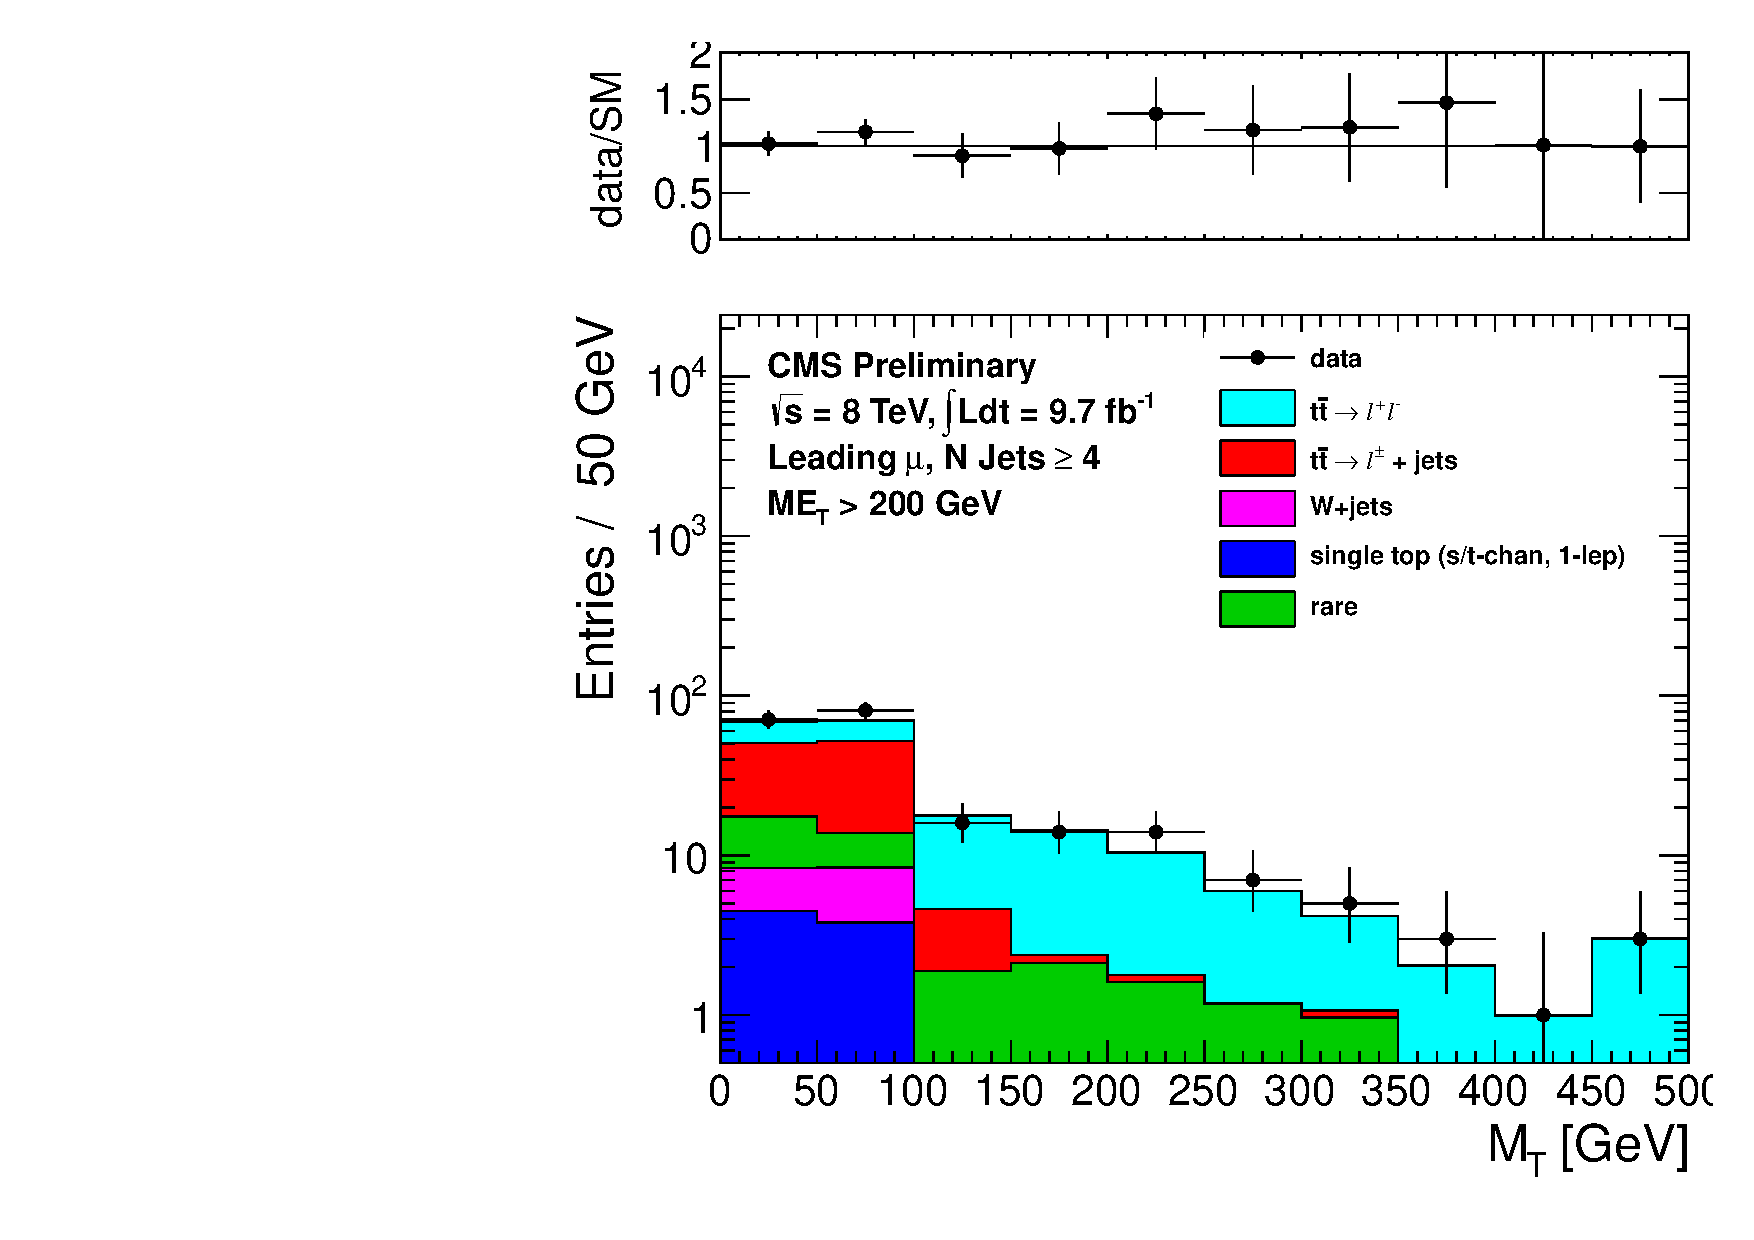
\includegraphics[width=0.5\linewidth]{plots/CR5plots/mt_met200_leadmuo_nj4.pdf}%
	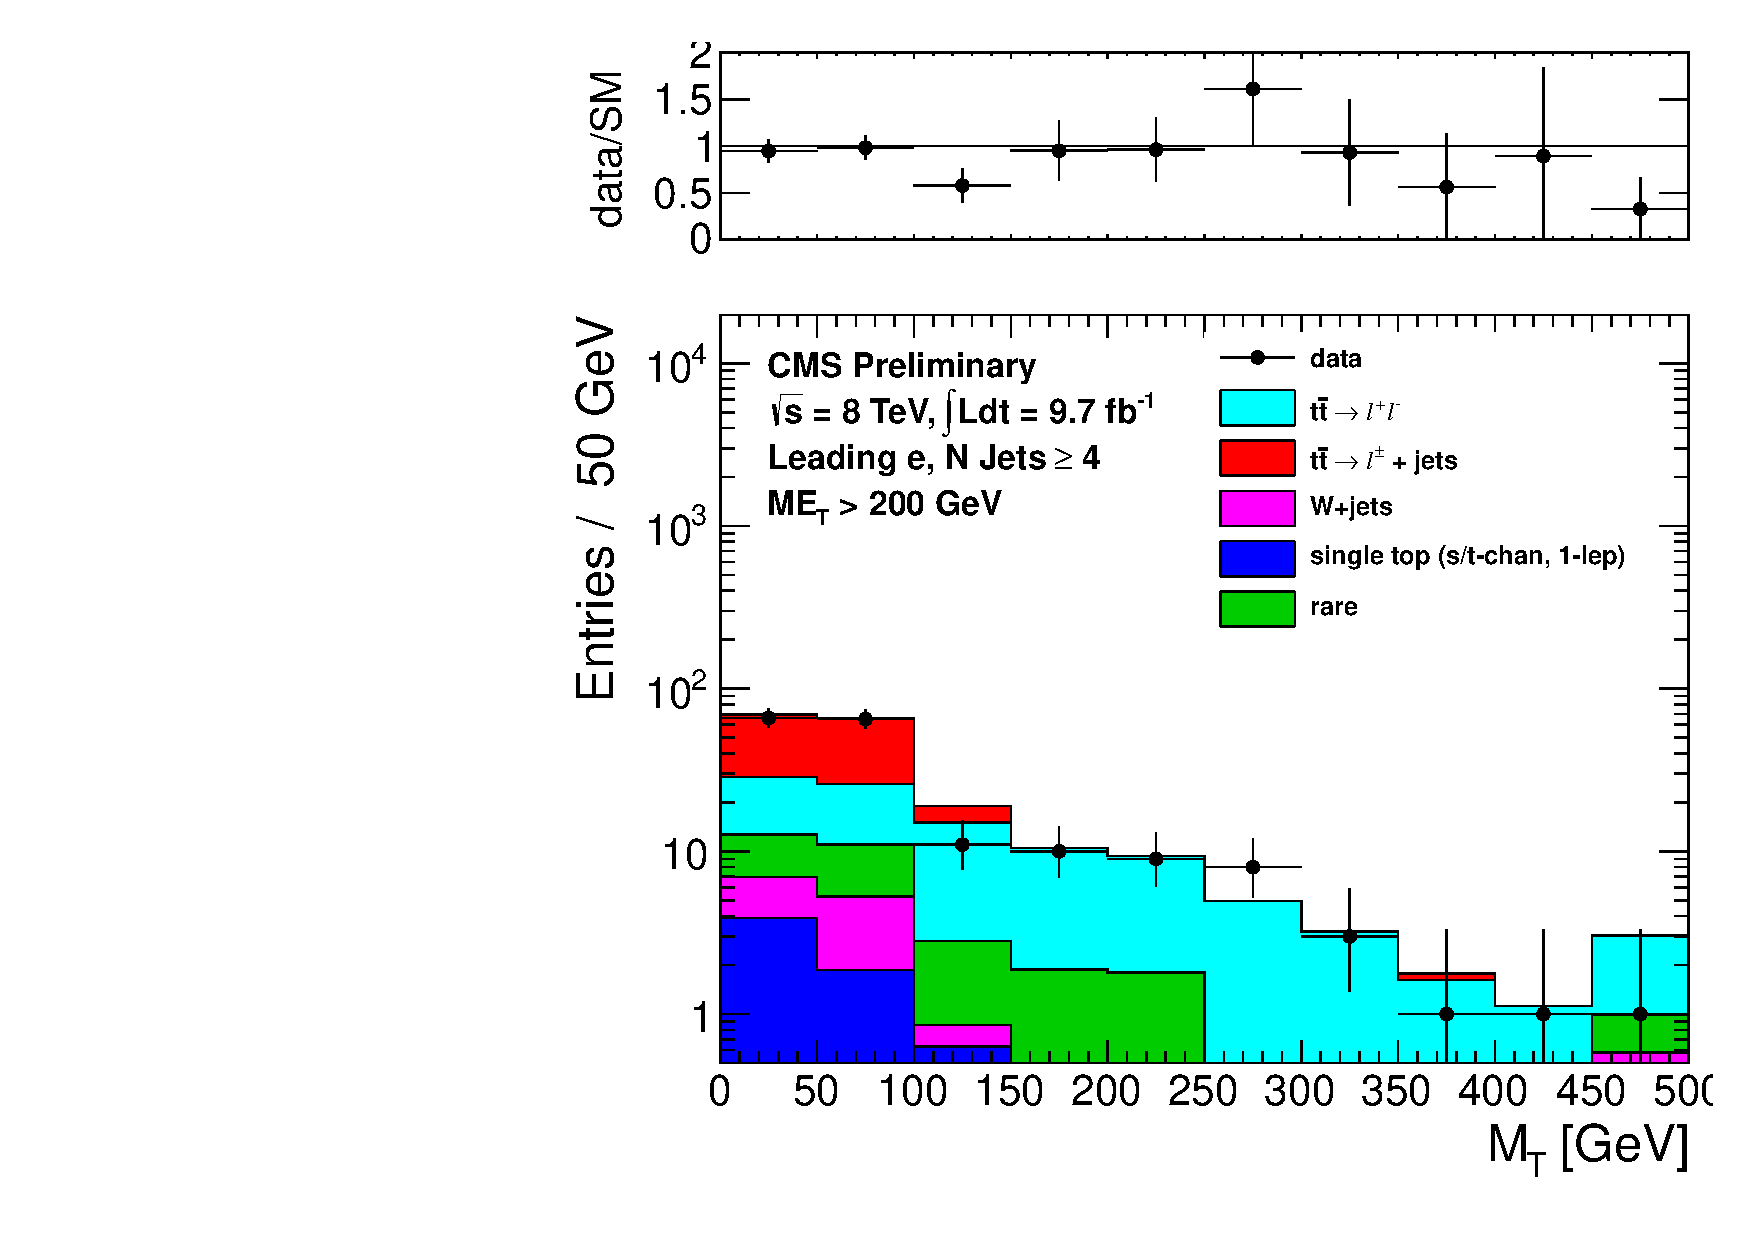
\includegraphics[width=0.5\linewidth]{plots/CR5plots/mt_met200_leadele_nj4.pdf}
	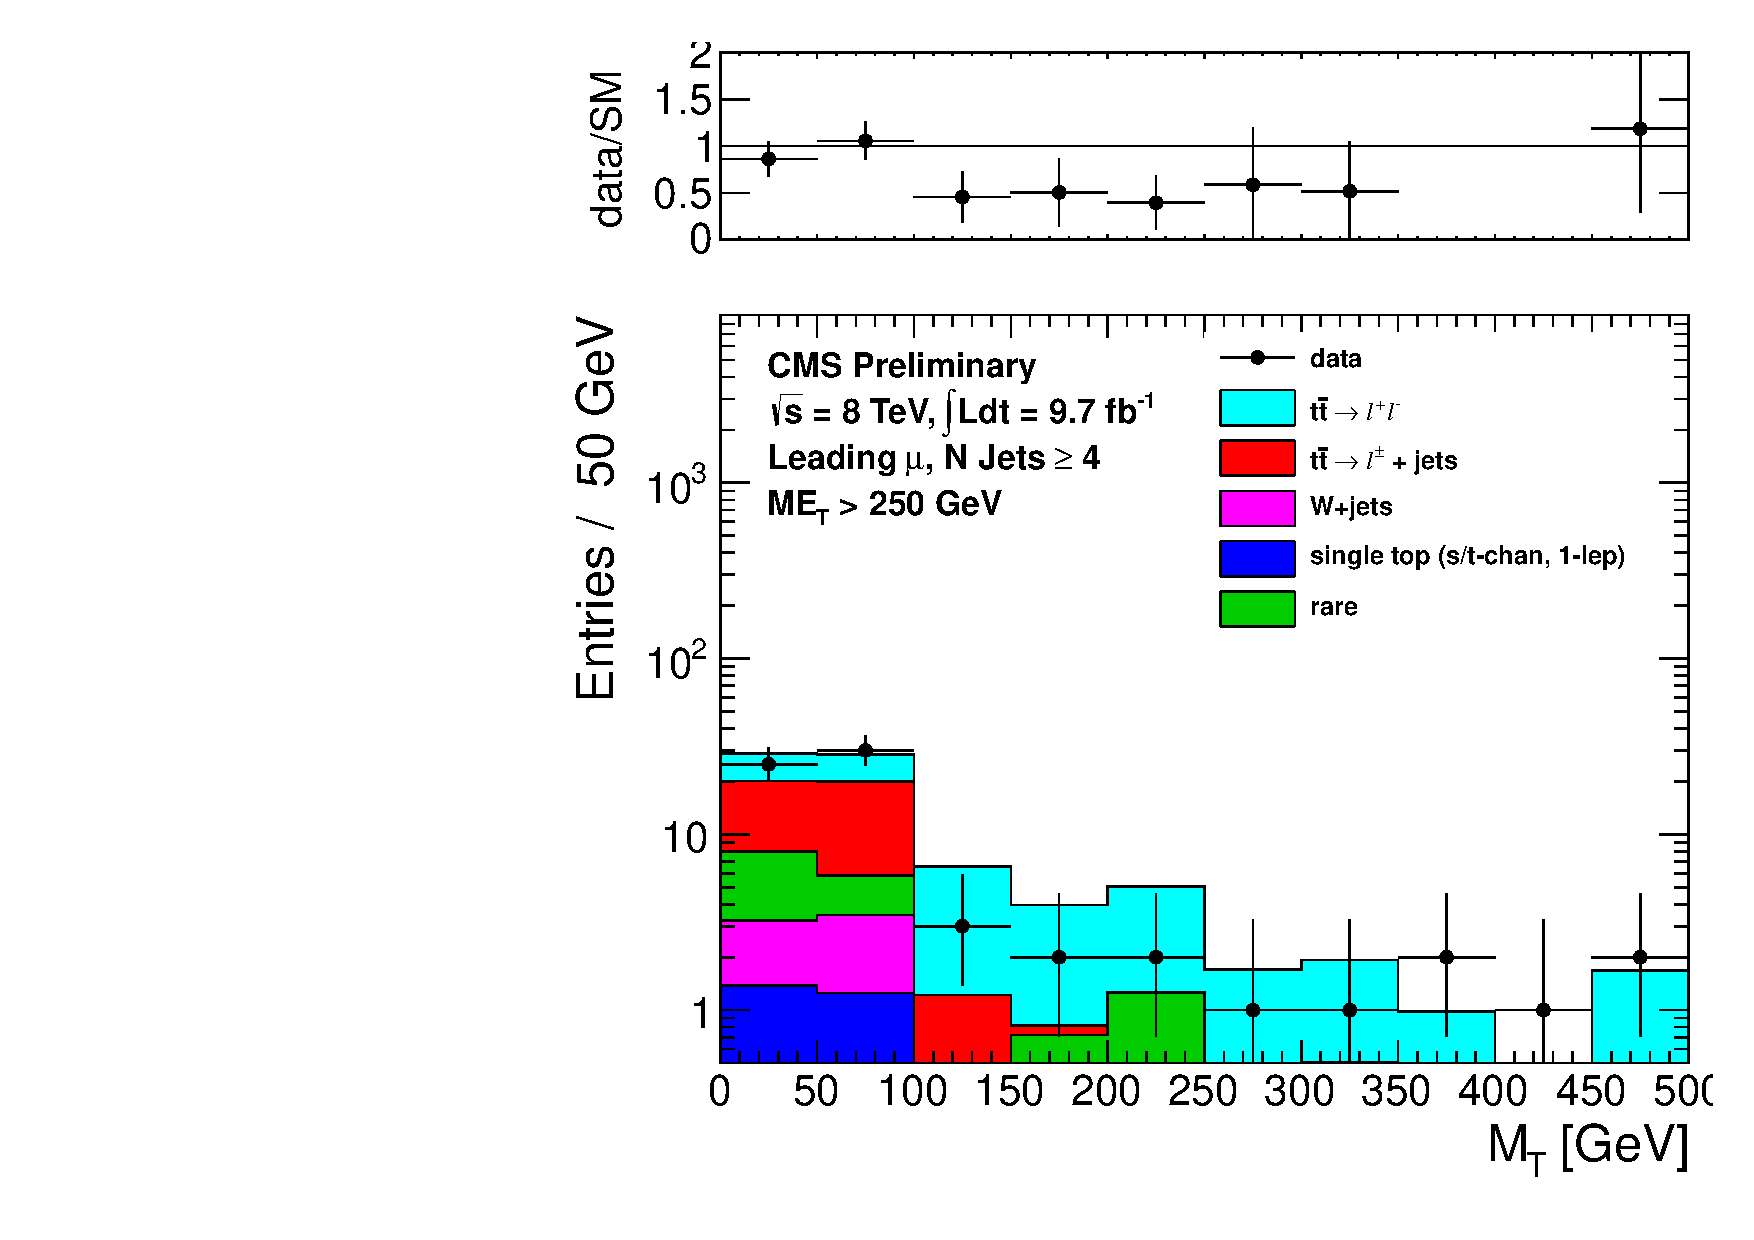
\includegraphics[width=0.5\linewidth]{plots/CR5plots/mt_met250_leadmuo_nj4.pdf}%
	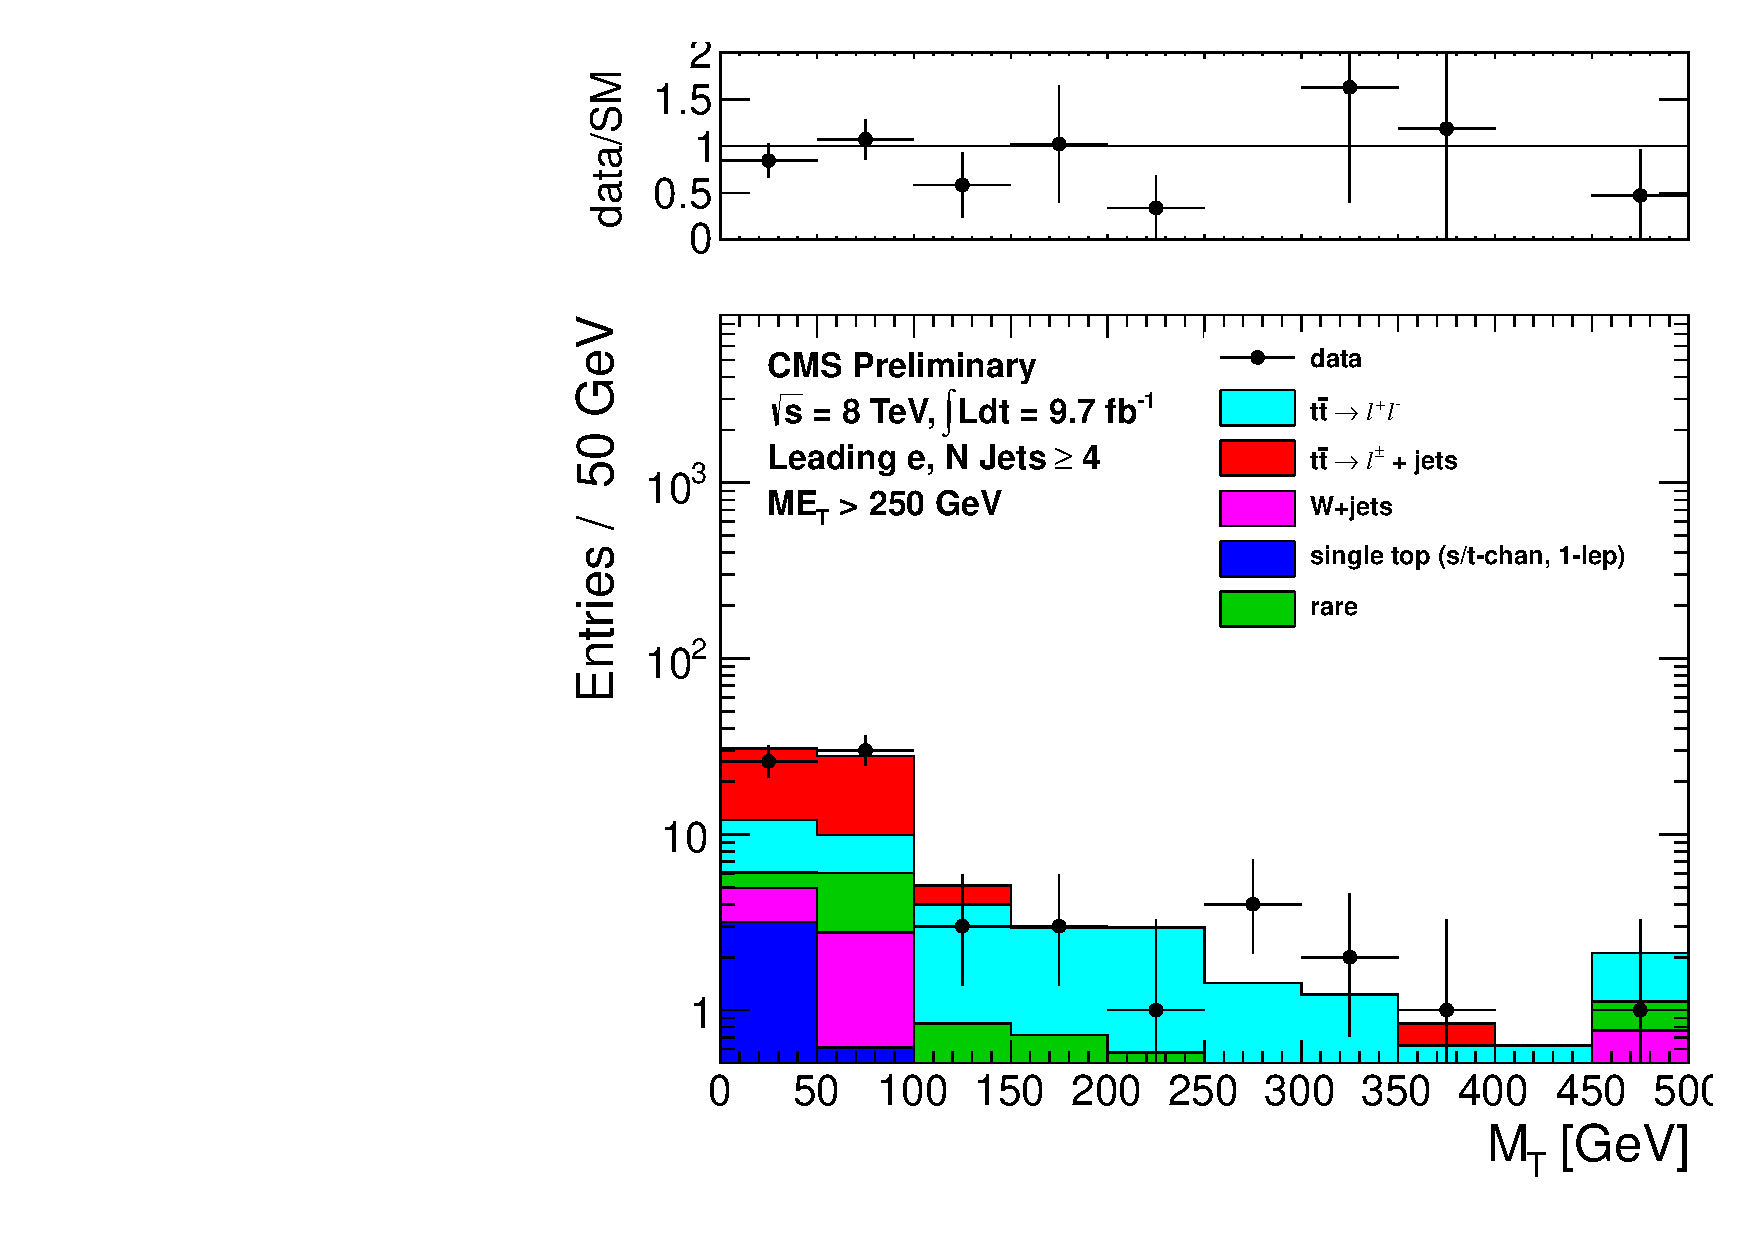
\includegraphics[width=0.5\linewidth]{plots/CR5plots/mt_met250_leadele_nj4.pdf}
    \caption{
      Comparison of the \mt\ distribution in data vs. MC for events
      with a leading muon (left) and leading electron (right)
      satisfying the requirements of CR5. The \met\ requirements used are
      150 GeV (top), 200 GeV (middle) and 250 GeV (bottom).
\label{fig:cr5mtrest} 
}  
      \end{center}
\end{figure}







